\documentclass[xelatex,aspectratio=169]{beamer}

\hfuzz=10pt
\vfuzz=10pt

% Theme
\usetheme{htw}
\setbeamertemplate{navigation symbols}{}
\setbeamertemplate{theorems}[numbered]
\setbeamercovered{transparent}

%\logo{
\includegraphics[height=0.5cm]{HTWD_color.png}}

% Packages
\usepackage{polyglossia}
\setmainlanguage{german}
\setotherlanguage{english}

\usepackage[bigfiles]{pdfbase}
\ExplSyntaxOn
\NewDocumentCommand\embedvideo{smm}{
\group_begin:
\leavevmode
\tl_if_exist:cTF{file_\file_mdfive_hash:n{#3}}{
  \tl_set_eq:Nc\video{file_\file_mdfive_hash:n{#3}}
}{
  \IfFileExists{#3}{}{\GenericError{}{File~`#3'~not~found}{}{}}
  \pbs_pdfobj:nnn{}{fstream}{{}{#3}}
  \pbs_pdfobj:nnn{}{dict}{
    /Type/Filespec/F~(#3)/UF~(#3)
    /EF~<</F~\pbs_pdflastobj:>>
  }
  \tl_set:Nx\video{\pbs_pdflastobj:}
  \tl_gset_eq:cN{file_\file_mdfive_hash:n{#3}}\video
}
%
\pbs_pdfobj:nnn{}{dict}{
  /Type/RichMediaInstance/Subtype/Video
  /Asset~\video
  /Params~<</FlashVars (
  source=#3&
  skin=SkinOverAllNoFullNoCaption.swf&
  skinAutoHide=true&
  skinBackgroundColor=0x5F5F5F&
  skinBackgroundAlpha=0.75
  )>>
}
%
\pbs_pdfobj:nnn{}{dict}{
/Type/RichMediaConfiguration/Subtype/Video
/Instances~[\pbs_pdflastobj:]
}
%
\pbs_pdfobj:nnn{}{dict}{
/Type/RichMediaContent
/Assets~<<
/Names~[(#3)~\video]
>>
/Configurations~[\pbs_pdflastobj:]
}
\tl_set:Nx\rmcontent{\pbs_pdflastobj:}
%
\pbs_pdfobj:nnn{}{dict}{
  /Activation~<<
  /Condition/\IfBooleanTF{#1}{PV}{XA}
  /Presentation~<</Style/Embedded>>
  >>
  /Deactivation~<</Condition/PI>>
}
%
\hbox_set:Nn\l_tmpa_box{#2}
\tl_set:Nx\l_box_wd_tl{\dim_use:N\box_wd:N\l_tmpa_box}
\tl_set:Nx\l_box_ht_tl{\dim_use:N\box_ht:N\l_tmpa_box}
\tl_set:Nx\l_box_dp_tl{\dim_use:N\box_dp:N\l_tmpa_box}
\pbs_pdfxform:nnnnn{1}{1}{}{}{\l_tmpa_box}
%
\pbs_pdfannot:nnnn{\l_box_wd_tl}{\l_box_ht_tl}{\l_box_dp_tl}{
  /Subtype/RichMedia
  /BS~<</W~0/S/S>>
  /Contents~(embedded~video~file:#3)
  /NM~(rma:#3)
  /AP~<</N~\pbs_pdflastxform:>>
  /RichMediaSettings~\pbs_pdflastobj:
  /RichMediaContent~\rmcontent
}
\phantom{#2}
\group_end:
}
\ExplSyntaxOff


\usepackage{graphicx}
\usepackage[export]{adjustbox}
\usepackage{animate}
%\usepackage[dvipdfmx]{movie15_dvipdfmx}
\usepackage{media9}
\usepackage{tabularx}
\usepackage{colortbl}
\usepackage{booktabs}
\usepackage{makecell}
\usepackage{ltablex}
\usepackage{array}
\usepackage{multirow}
\usepackage{amsmath}
\usepackage{amsthm}
%\renewcommand{\arraystretch}{1.5}
\newcolumntype{L}[1]{>{\raggedright\let\newline\\\arraybackslash\hspace{0pt}}p{#1}}
\newcolumntype{C}[1]{>{\centering\let\newline\\\arraybackslash\hspace{0pt}}p{#1}}
\newcolumntype{R}[1]{>{\raggedleft\let\newline\\\arraybackslash\hspace{0pt}}p{#1}}
%\renewcommand\thesatz{\arabic{section}.\arabic{theorem}}
\makeatletter
\@addtoreset{theorem}{lecture}
\makeatother

\newtheorem{satz}{Satz}[section]
\newtheorem{lem}{Lemma}[section]
\newtheorem{beh}{Behauptung}[section]
\newtheorem{define}{Definition}[section]
\numberwithin{equation}{section}
\usepackage{ragged2e}
\usepackage{etoolbox}

\usepackage{color}
\usepackage{colortbl}
\definecolor{hellgrau}{rgb}{0.85,0.85,0.85}
\definecolor{hellrot}{rgb}{1,0.7,0.7}

\usepackage{tikz}
\usetikzlibrary{shapes,arrows.meta,calc,arrows,positioning,patterns,tikzmark}
%\usepackage{tikz-uml}
\usepackage{pgfplots}  % for elliptic curves (part 8)
\pgfplotsset{compat=1.18}
\usepackage{pgffor}
\usepackage{pgfmath-xfp}
\tikzset{>=latex}
\tikzset{
  invisible/.style={opacity=0},
  visible on/.style={alt={#1{}{invisible}}},
  alt/.code args={<#1>#2#3}{%
      \alt<#1>{\pgfkeysalso{#2}}{\pgfkeysalso{#3}} % \pgfkeysalso doesn't change the path
    },
}

\usepackage{paralist}

\usepackage{url}
\def\UrlBreaks{\do\/\do-}
\PassOptionsToPackage{hyphens}{url}\usepackage{hyperref}

\usepackage[normalem]{ulem} % gestrichelte Unterstreichung (\dashuline{})
\usepackage{cancel}

\makeatletter
\renewcommand{\itemize}[1][]{%
  \beamer@ifempty{#1}{}{\def\beamer@defaultospec{#1}}%
  \ifnum \@itemdepth >2\relax\@toodeep\else
    \advance\@itemdepth\@ne
    \beamer@computepref\@itemdepth% sets \beameritemnestingprefix
    \usebeamerfont{itemize/enumerate \beameritemnestingprefix body}%
    \usebeamercolor[fg]{itemize/enumerate \beameritemnestingprefix body}%
    \usebeamertemplate{itemize/enumerate \beameritemnestingprefix body begin}%
    \list
    {\usebeamertemplate{itemize \beameritemnestingprefix item}}
    {\def\makelabel##1{%
        {%
            \hss\llap{{%
                  \usebeamerfont*{itemize \beameritemnestingprefix item}%
                  \usebeamercolor[fg]{itemize \beameritemnestingprefix item}##1}}%
          }%
      }%
    }
  \fi%
  \beamer@cramped%
  \justifying% NEW
  %\raggedright% ORIGINAL
  \beamer@firstlineitemizeunskip%
}
\makeatother

\apptocmd{\frame}{}{\justifying}{}

\renewcommand\theadfont{\bfseries\sffamily}
\usepackage{ragged2e}
\usepackage{newpxtext}

\setsansfont{texgyreheros}[
  Scale=MatchLowercase,
  UprightFont=*-regular,
  BoldFont=*-bold,
  ItalicFont=*-italic,
  BoldItalicFont=*-bolditalic,
]

% Title
\usepackage[usetransparent=false]{svg}
% Import references
\usepackage[backend=biber,style=numeric,sorting=none]{biblatex}
\addbibresource{references.bib}

%\AtBeginSection[]{
%  \begin{frame}
%    \vfill
%    \centering
%    \begin{beamercolorbox}[sep=8pt,center,shadow=true,rounded=true]{title}
%      \usebeamerfont{title}\thesection.~\secname\par%
%    \end{beamercolorbox}
%    \vfill
%  \end{frame}
%}

\makeatletter
\newenvironment{noheadline}{
  \setbeamertemplate{headline}{}
  \addtobeamertemplate{frametitle}{\vspace*{-0.9\baselineskip}}{}
}{}
\makeatother


\usepackage{xcolor}
\usepackage{algorithm}
\usepackage[linesnumbered,ruled,lined,commentsnumbered,algo2e,ngerman,ngermankw]{algorithm2e}
\usepackage{algorithmic}
\usepackage{caption}
\usepackage[newfloat]{minted}
\captionsetup[listing]{position=top}
\definecolor{mintedbg}{HTML}{282828}
\setminted{
  breaklines=true,
  bgcolor=mintedbg,
  style=monokai,
  formatcom=\color{white}
}
\usepackage{etoolbox}
\makeatletter
% replace \medskip before and after the box with nothing, i.e., remove it
\patchcmd{\minted@colorbg}{\medskip}{}{}{}
\patchcmd{\endminted@colorbg}{\medskip}{}{}{}
\makeatother

\renewcommand{\theFancyVerbLine}{\textcolor{black}{\arabic{FancyVerbLine}}}

\usepackage{pifont}
\newcommand{\cmark}{\ding{51}}%
\newcommand{\xmark}{\ding{55}}%

\newenvironment{changemargin}[2]{%
  \begin{list}{}{%
      \setlength{\topsep}{0pt}%
      \setlength{\leftmargin}{#1}%
      \setlength{\rightmargin}{#2}%
      \setlength{\listparindent}{\parindent}%
      \setlength{\itemindent}{\parindent}%
      \setlength{\parsep}{\parskip}%
    }%
    \item[]}{\end{list}}


\usepackage{csquotes}

% Title
\title{Zahlensysteme}
\author{Prof. Dr. Lukas Iffländer}
\institute{HTW Dresden}
\date{}
\usepackage{svg}

% Begin document
\begin{document}

% Title slide
\begin{frame}
  \titlepage
\end{frame}

\section{Probleme}

\begin{frame}{Probleme durch Computerarithmetik}{Beispiele}
  \begin{columns}
    \begin{column}{0.5\textwidth}
      
\includegraphics[width=\textwidth]{img/ariane_crash.png}
    \end{column}
    \begin{column}{0.5\textwidth}
      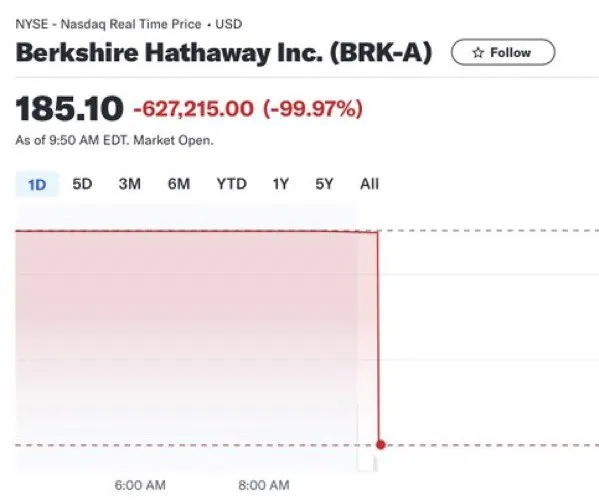
\includegraphics[width=\textwidth]{img/berkshire_crash.png}
    \end{column}
  \end{columns}
\end{frame}

\begin{frame}{Probleme durch Computerarithmetik}{Integer Overflow}
  \begin{columns}
    \begin{column}{0.6\textwidth}
      \small
      \inputminted{c}{src/zahlensysteme_ueberlauf.c}
    \end{column}
    \begin{column}{0.4\textwidth}
      Ausgabe:

      \texttt{Max int value: 2147483647} \\
      \texttt{After overflow: -2147483648}
    \end{column}
  \end{columns}
\end{frame}

\section{Überblick}

\begin{frame}{Zahlensysteme}
  \begin{itemize}
    \item Ein Zahlensystem legt die jeweiligen Regeln fest, wie Zahlen als Ziffernfolge dargestellt werden können \textrightarrow Anordnung der Ziffern festlegen
    \item Ein Zahlensystem legt fest, welcher Wert einer Ziffernfolge zugeordnet ist (A = 10, 1010 = 10 usw.) \textrightarrow Vorschrift zur Ermittlung des Zahlenwerts festlegen
    \item (Gleiche) Zahlen lassen sich in unterschiedlichen Zahlensystemen in verschiedener Form darstellen
  \end{itemize}

  \begin{block}{Unterscheidung}
    \begin{itemize}
      \item Additionssysteme
      \item Stellenwertsysteme (Positionssysteme)
      \item Hybrid-Systeme
    \end{itemize}
  \end{block}
\end{frame}

\begin{frame}{Additionssysteme}
  \begin{itemize}
    \item Jede Ziffer hat einen festen Wert
    \item Der Wert einer Ziffernfolge ergibt sich aus der Summe der Werte der einzelnen Ziffern
          \begin{exampleblock}{Unärsystem}
            Im Unärsystem wird jede Zahl durch eine wiederholte Ziffer dargestellt. Zum Beispiel wird die Zahl 3 als 111 dargestellt.
          \end{exampleblock}
          \begin{exampleblock}{Römische Zahlen}
            Die römischen Zahlen sind ein Additionssystem. Die Ziffern I, V, X, L, C, D und M haben die Werte 1, 5, 10, 50, 100, 500 und 1000.

            Besonderheit: Die Ziffernfolge wird von links nach rechts gelesen. Ist eine Ziffer kleiner als die nächste, wird sie subtrahiert.

            Beispiel: Die Zahl IX wird als 9 interpretiert, da I (1) vor X (10) steht.
          \end{exampleblock}
  \end{itemize}
\end{frame}

\begin{frame}{Stellenwertsysteme}
  \begin{itemize}
    \item Jede Ziffer hat einen festen Wert
    \item Der Wert einer Ziffernfolge ergibt sich aus der Summe der Produkte der Ziffern mit den zugehörigen Potenzen der Basis
          \begin{exampleblock}{Dezimalsystem}
            Im Dezimalsystem haben die Ziffern die Werte 0 bis 9. Die Basis ist 10.

            Beispiel: Die Zahl 1234 wird als $1 \cdot 10^3 + 2 \cdot 10^2 + 3 \cdot 10^1 + 4 \cdot 10^0 = 1234$ interpretiert.
          \end{exampleblock}
          \begin{exampleblock}{Binärsystem}
            Im Binärsystem haben die Ziffern die Werte 0 und 1. Die Basis ist 2.

            Beispiel: Die Zahl 1011 wird als $1 \cdot 2^3 + 0 \cdot 2^2 + 1 \cdot 2^1 + 1 \cdot 2^0 = 11$ interpretiert.
          \end{exampleblock}
  \end{itemize}
\end{frame}

\begin{frame}{Stellenwertsysteme}{Darstellung natürlicher Zahlen}
  In der Informatik verwenden wir in der Regel vier Zahlensysteme:
  \begin{table}
    \begin{tabular}{lrrr}
      \toprule
      System            & Basis & Ziffern                                        & Beispiel \\
      \midrule
      Binärsystem       & 2     & 0, 1                                           & 1011     \\
      Oktalsystem       & 8     & 0, 1, 2, 3, 4, 5, 6, 7                         & 1234     \\
      Dezimalsystem     & 10    & 0, 1, 2, 3, 4, 5, 6, 7, 8, 9                   & 1234     \\
      Hexadezimalsystem & 16    & 0, 1, 2, 3, 4, 5, 6, 7, 8, 9, A, B, C, D, E, F & 4D2      \\
      \bottomrule
    \end{tabular}
  \end{table}
\end{frame}

\begin{frame}{Stellenwertsysteme}{Unterscheidung (Mathematik)}
  \textbf{Welchen Wert hat 1010?}

  In der Informatik ist es wichtig, die Basis des Zahlensystems zu kennen, um den Wert einer Ziffernfolge zu bestimmen.

  \begin{block}{Konvention}
    Zur eindeutigen Darstellung von Zahlen in verschiedenen Zahlensystemen wird die Basis oft als Index hinter der Zahl geschrieben. Zum Beispiel wird die Zahl 1010 im Binärsystem als $1010_2$ und im Dezimalsystem als $1010_{10}$ dargestellt.
  \end{block}

\end{frame}

\begin{frame}{Stellenwertsysteme}{Unterscheidung}
  \textbf{Wie mache ich denn einen Index in Python?}

  Antwort: Gar nicht. Stattdessen gibt es unterschiedliche Möglichkeiten, Python zu sagen, dass eine Zahl in einem bestimmten Zahlensystem dargestellt ist.

  \begin{table}
    \begin{tabular}{ll}
      \toprule
      Zahlensystem & Darstellung in Python \\
      \midrule
      Binär        & \texttt{0b1010}       \\
      Oktal        & \texttt{0o1234}       \\
      Dezimal      & \texttt{1234}         \\
      Hexadezimal  & \texttt{0x4D2}        \\
      \bottomrule
    \end{tabular}
  \end{table}
\end{frame}

\begin{frame}{Stellenwertsysteme}{Darstellung}
  \begin{columns}
    \begin{column}{0.5\textwidth}
      \begin{itemize}
        \item natürliche Zahlen

              \( \mathbb{N} = \{1, 2, \ldots\} \)
        \item ganze Zahlen

              \( \mathbb{Z} = \{\ldots, -2, -1, 0, 1, 2, \ldots\} \)
        \item rationale Zahlen

              \( \mathbb{Q} = \left\{\frac{a}{b} \mid a, b \in \mathbb{Z}, b \neq 0\right\} \)
        \item reelle Zahlen

              \( \mathbb{R} \)
      \end{itemize}
    \end{column}
    \begin{column}{0.5\textwidth}
      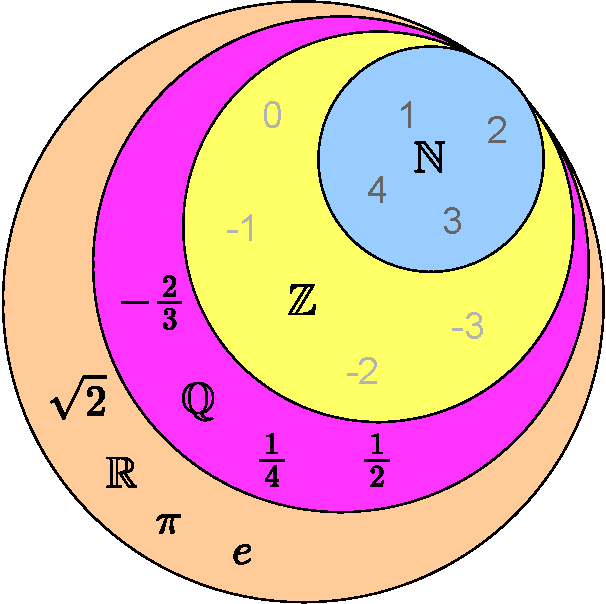
\includegraphics[width=.8\textwidth]{img/zahlensysteme_mengen.pdf}
    \end{column}
  \end{columns}

\end{frame}

\begin{frame}{Stellenwertsysteme}{Darstellung natürlicher Zahlen}
  \begin{columns}
    \begin{column}{0.5\textwidth}
      \begin{block}{Darstellung als Potenz}
        Jede natürliche Zahl \(n\) lässt sich als eine Summe von Potenzen einer beliebigen anderen natürlichen Zahl \(B \geq 2 \) darstellen in der Form
        \[
          n = \sum_{i=0}^{N-1} z_i \cdot B^i
        \]
        darstellen
        \begin{itemize}
          \item \(B\) = Basis des Zahlensystems (\(B \geq 2\))
          \item \(z_i\) = i-te Ziffer der Darstellung (\(0 \leq z_i < B\))
          \item \(N\) = Anzahl der Ziffern
        \end{itemize}
      \end{block}
    \end{column}
    \begin{column}{0.5\textwidth}
      \begin{tabularx}{\textwidth}{lrX}
        \toprule
        System            & Basis & Ziffern                                        \\
        \midrule
        Binär             & 2     & 0, 1                                           \\
        Oktalsystem       & 8     & 0, 1, 2, 3, 4, 5, 6, 7                         \\
        Dezimalsystem     & 10    & 0, 1, 2, 3, 4, 5, 6, 7, 8, 9                   \\
        Hexadezimalsystem & 16    & 0, 1, 2, 3, 4, 5, 6, 7, 8, 9, A, B, C, D, E, F \\
        \bottomrule
      \end{tabularx}
    \end{column}
  \end{columns}
\end{frame}

\begin{frame}{Stellenwertsysteme}{Darstellung natürlicher Zahlen}
  \begin{columns}
    \begin{column}{0.5\textwidth}
      \begin{block}{Darstellung als Potenz}
        Jede natürliche Zahl \(n\) lässt sich als eine Summe von Potenzen einer beliebigen anderen natürlichen Zahl \(B \geq 2 \) darstellen in der Form
        \[
          n = \sum_{i=0}^{N-1} z_i \cdot B^i
        \]
        darstellen
        \begin{itemize}
          \item \(B\) = Basis des Zahlensystems (\(B \geq 2\))
          \item \(z_i\) = i-te Ziffer der Darstellung (\(0 \leq z_i < B\))
          \item \(N\) = Anzahl der Ziffern
        \end{itemize}
      \end{block}
    \end{column}
    \begin{column}{0.5\textwidth}
      \begin{exampleblock}{Beispiel: Dezimalsystem}
        \smaller
        \begin{align*}
          2021 & = \sum_{i=0}^{3} z_i \cdot 10^i                                     \\
               & = z_0 \cdot 10^0 + z_1 \cdot 10^1 + z_2 \cdot 10^2 + z_3 \cdot 10^3 \\
               & = 1 \cdot 10^0 + 2 \cdot 10^1 + 0 \cdot 10^2 + 2 \cdot 10^3         \\
               & = 1 \cdot 1 + 2 \cdot 10 + 0 \cdot 100 + 2 \cdot 1000               \\
               & = 1 + 20 + 0 + 2000                                                 \\
               & = 2021_{10}
        \end{align*}
      \end{exampleblock}
    \end{column}
  \end{columns}
\end{frame}

\begin{frame}{Stellenwertsysteme}{Darstellung natürlicher Zahlen}
  \begin{columns}
    \begin{column}{0.5\textwidth}
      \begin{block}{Darstellung als Potenz}
        Jede natürliche Zahl \(n\) lässt sich als eine Summe von Potenzen einer beliebigen anderen natürlichen Zahl \(B \geq 2 \) darstellen in der Form
        \[
          n = \sum_{i=0}^{N-1} z_i \cdot B^i
        \]
        darstellen
        \begin{itemize}
          \item \(B\) = Basis des Zahlensystems (\(B \geq 2\))
          \item \(z_i\) = i-te Ziffer der Darstellung (\(0 \leq z_i < B\))
          \item \(N\) = Anzahl der Ziffern
        \end{itemize}
      \end{block}
    \end{column}
    \begin{column}{0.5\textwidth}
      \begin{exampleblock}{Beispiel: Binärsystem}
        \smaller
        \begin{align*}
          10110 & = \sum_{i=0}^{4} z_i \cdot 2^i                                                  \\
                & = z_0 \cdot 2^0 + z_1 \cdot 2^1 + z_2 \cdot 2^2 + z_3 \cdot 2^3 + z_4 \cdot 2^4 \\
                & = 0 \cdot 2^0 + 1 \cdot 2^1 + 1 \cdot 2^2 + 0 \cdot 2^3 + 1 \cdot 2^4           \\
                & = 0 \cdot 1 + 1 \cdot 2 + 1 \cdot 4 + 0 \cdot 8 + 1 \cdot 16                    \\
                & = 0 + 2 + 4 + 0 + 16                                                            \\
                & = 22_{10}
        \end{align*}
      \end{exampleblock}
    \end{column}
  \end{columns}
\end{frame}

\begin{frame}{Stellenwertsysteme}{Darstellung natürlicher Zahlen}
  \begin{columns}
    \begin{column}{0.5\textwidth}
      \begin{block}{Darstellung als Potenz}
        Jede natürliche Zahl \(n\) lässt sich als eine Summe von Potenzen einer beliebigen anderen natürlichen Zahl \(B \geq 2 \) darstellen in der Form
        \[
          n = \sum_{i=0}^{N-1} z_i \cdot B^i
        \]
        darstellen
        \begin{itemize}
          \item \(B\) = Basis des Zahlensystems (\(B \geq 2\))
          \item \(z_i\) = i-te Ziffer der Darstellung (\(0 \leq z_i < B\))
          \item \(N\) = Anzahl der Ziffern
        \end{itemize}
      \end{block}
    \end{column}
    \begin{column}{0.5\textwidth}
      \begin{exampleblock}{Beispiel: Hexadezimalsystem}
        \smaller
        \begin{align*}
          1C & = \sum_{i=0}^{1} z_i \cdot 16^i   \\
             & = z_0 \cdot 16^0 + z_1 \cdot 16^1 \\
             & = 12 \cdot 16^0 + 1 \cdot 16^1    \\
             & = 12 \cdot 1 + 1 \cdot 16         \\
             & = 12 + 16                         \\
             & = 28_{10}
        \end{align*}
      \end{exampleblock}
    \end{column}
  \end{columns}
\end{frame}

\begin{frame}{Stellenwertsysteme}{Darstellung von Wertebereichen}
  \begin{columns}
    \begin{column}{0.3\textwidth}
      \begin{block}{Zahlenkreis (endlich)}
        \centering
        \resizebox{\textwidth}{!}{
          \begin{tikzpicture}[rotate=90]

            \draw[thick] (0:3cm) arc (0:-360:3cm);
            \foreach \i in {0,...,3}
              {
                \draw(-\i * 20:3cm) -- (-\i * 20:3.5cm) node[above] {\i};
              }
            \foreach \i in {4,...,18}
              {
                \draw(-\i * 20:3cm) -- (-\i * 20:3.5cm) node[right] {};
              }
            \draw(1 * 20:3cm) -- (1 * 20:3.5cm) node[above] {$B^n -1$};
            \draw(2 * 20:3cm) -- (2 * 20:3.5cm) node[above] {$B^n -2$};
          \end{tikzpicture}
        }
      \end{block}
    \end{column}
    \begin{column}{0.7\textwidth}
      \begin{alertblock}{Problem}
        Während die natürlichen Zahlen unendlich sind, können wir in technischen Systemen nur mit endlichen Zahlen arbeiten.
      \end{alertblock}
      \begin{block}{Eigenschaft}
        Die Repräsentation von Zahlen in einem Computer ist immer auf eine gewisse Anzahl von Bits (Stellen im Binärsystem) beschränkt.
      \end{block}
      \begin{exampleblock}{Beispiele}
        \centering
        \begin{tabular}{cccc}
          \toprule
          \textbf{Basis} & \textbf{Stellen} & \textbf{Zahlen} & \textbf{Werte}                   \\
          \midrule
          10             & 3                & $10^3$ = 1000   & {000, 001, 002, \ldots~998, 999} \\
          2              & 3                & $2^3$ = 8       & {000, 001, 010, \ldots~110, 111} \\
          \bottomrule
        \end{tabular}
      \end{exampleblock}

    \end{column}

  \end{columns}

\end{frame}

\begin{frame}{Binärzahl und Dualzahl}
  \begin{alertblock}{Besonderheit der deutschen Sprache}
    \begin{center}
      Binärzahl $\not\equiv$ Dualzahl
    \end{center}

    Die Begriffe Dual- und Binärzahl werden oft synonym verwendet. In der deutschen Sprache sind die Begriffe jedoch voneinander abzugrenzen (im Gegensatz zur englischen Sprache \enquote{dual number} und \enquote{binary number} werden synonym verwendet).
  \end{alertblock}
  \begin{columns}[onlytextwidth]
    \begin{column}{0.48\textwidth}
      \begin{block}{Binärzahl}
        Zur Darstellung werden zwei beliebige Zeichen verwenden. (z. B. 0 und 1 oder + und -)
      \end{block}
    \end{column}
    \begin{column}{0.48\textwidth}
      \begin{block}{Dualzahl}
        Zahl in einem Stellenwertsystem zur Basis 2. (Ziffern 0 und 1).
      \end{block}
    \end{column}
  \end{columns}
  \begin{block}{Regel}
    \begin{center}
      Dualzahl $\rightarrow$ Binärzahl
    \end{center}
  \end{block}
\end{frame}

\section{Konvertierung}

\begin{frame}{Konvertierung natürlicher Zahlen}{Wege}
  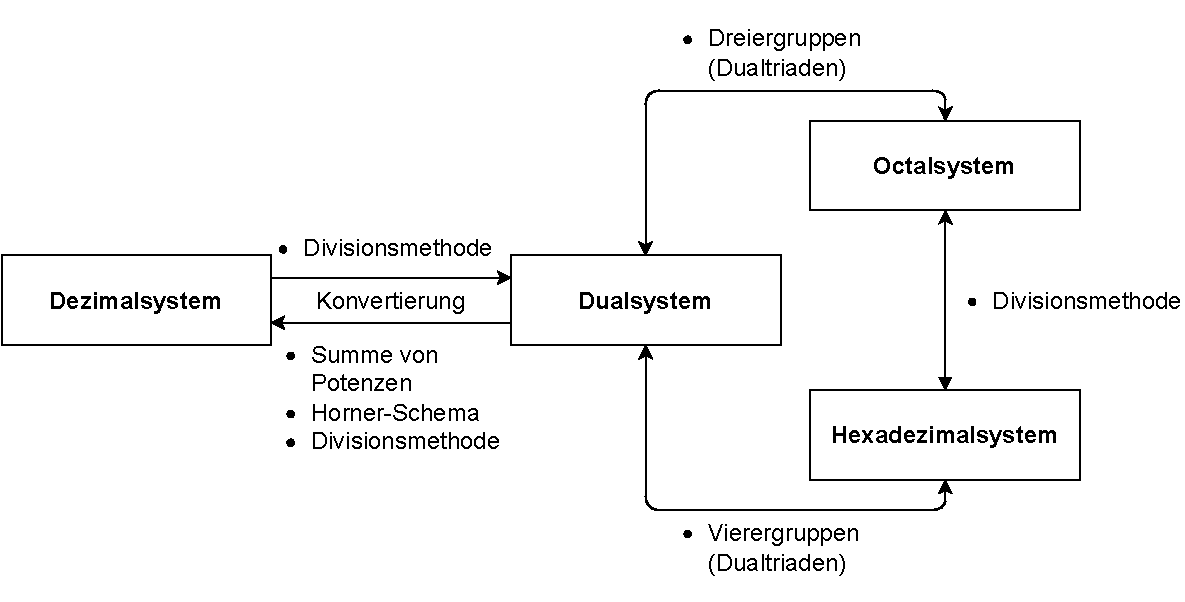
\includegraphics[width=\textwidth]{fig/zahlensysteme_umwandlung.pdf}
\end{frame}

\begin{frame}{Konvertierung natürlicher Zahlen}{Wege (Wertebeispiel)}
  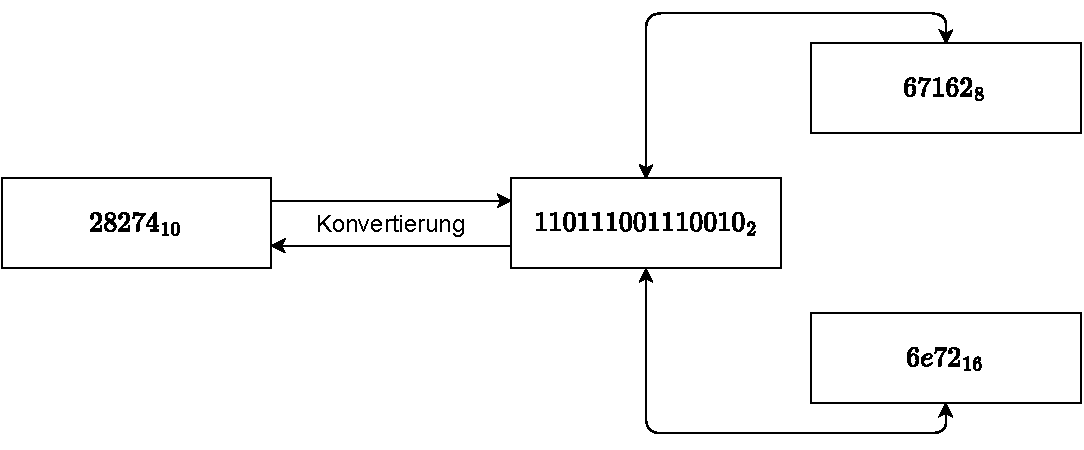
\includegraphics[width=\textwidth]{fig/zahlensysteme_umwandlung_werte.pdf}
\end{frame}

\begin{frame}{Divisionsmethode}
  \begin{block}{Grundidee}
    \begin{itemize}
      \item Eine Zahl $z$ aus einem Stellenwertsystem $Q$ mit der Basis $p$ wird durch fortgesetzte Division mit Rest mit $q$ in eine Zahl $z^{'}$ im Stellenwertsystem $Z$ mit der Basis $q$ konvertiert.
      \item Die Rechnung (Division) findet im Quellsystem statt ($q$ ist somit auch im Quellsystem darzustellen)
      \item Die Divisionsreste werden im Zielsystem dargestellt
    \end{itemize}
  \end{block}
  \begin{block}{Algorithmus}
    \begin{enumerate}
      \item $x = \floor*{\frac{z}{q}}$, y = $z \mod q$, speichere $y$
      \item $z = x$
      \item Wiederhole 1. und 2. bis $x = 0$
      \item Schreibe die gespeicherten Reste in umgekehrter Reihenfolge auf.
    \end{enumerate}

  \end{block}

\end{frame}

\begin{frame}{Divisionsmethode}{Beispiel: Dezimalzahl nach Dualzahl}
  \begin{center}
    \begin{tabular}{rcrcrcr}
      \toprule
      \textbf{Dezimalzahl $z$} & : & \textbf{2} & = & $x$  & Rest & $y$                             \\
      \midrule
      2020                     & : & 2          & = & 1010 & Rest & 0\tikzmark{division_dual_first} \\
      1010                     & : & 2          & = & 505  & Rest & 0                               \\
      505                      & : & 2          & = & 252  & Rest & 1                               \\
      252                      & : & 2          & = & 126  & Rest & 0                               \\
      126                      & : & 2          & = & 63   & Rest & 0                               \\
      63                       & : & 2          & = & 31   & Rest & 1                               \\
      31                       & : & 2          & = & 15   & Rest & 1                               \\
      15                       & : & 2          & = & 7    & Rest & 1                               \\
      7                        & : & 2          & = & 3    & Rest & 1                               \\
      3                        & : & 2          & = & 1    & Rest & 1                               \\
      1                        & : & 2          & = & 0    & Rest & 1\tikzmark{division_dual_last}  \\
      \bottomrule
    \end{tabular}
  \end{center}
  \begin{tikzpicture}[overlay, remember picture]
    \draw[->, line width=1.5pt] ([yshift=0,xshift=1em] pic cs:division_dual_last) -- ([yshift=.7\baselineskip,xshift=1em] pic cs:division_dual_first);
    \path (pic cs:division_dual_first) -- (pic cs:division_dual_last) coordinate[midway] (midpoint_dual);
    \node[right=1em] at (midpoint_dual) {$111~1110~0100$};
  \end{tikzpicture}

\end{frame}

\begin{frame}{Divisionsmethode}{Beispiel: Dezimalzahl nach Oktalzahl}
  \begin{center}
    \begin{tabular}{rcrcrcr}
      \toprule
      \textbf{Dezimalzahl $z$} & : & \textbf{8} & = & $x$ & Rest & $y$                              \\
      \midrule
      2020                     & : & 8          & = & 252 & Rest & 4\tikzmark{division_octal_first} \\
      252                      & : & 8          & = & 31  & Rest & 4                                \\
      31                       & : & 8          & = & 3   & Rest & 7                                \\
      3                        & : & 8          & = & 0   & Rest & 3\tikzmark{division_octal_last}  \\
      \bottomrule
    \end{tabular}
  \end{center}
  \begin{tikzpicture}[overlay, remember picture]
    \draw[->, line width=1.5pt] ([yshift=0,xshift=1em] pic cs:division_octal_last) -- ([yshift=.7\baselineskip,xshift=1em] pic cs:division_octal_first);
    \path (pic cs:division_octal_first) -- (pic cs:division_octal_last) coordinate[midway] (midpoint_octal);
    \node[right=1em] at (midpoint_octal) {$3744$};

  \end{tikzpicture}
\end{frame}

\begin{frame}{Divisionsmethode}{Beispiel: Dezimalzahl nach Hexadezimalzahl}
  \begin{center}
    \begin{tabular}{rcrcrcr}
      \toprule
      \textbf{Dezimalzahl $z$} & : & \textbf{16} & = & $x$ & Rest & $y$                            \\
      \midrule
      2020                     & : & 16          & = & 126 & Rest & 4\tikzmark{division_hex_first} \\
      126                      & : & 16          & = & 7   & Rest & 14                             \\
      7                        & : & 16          & = & 0   & Rest & 7\tikzmark{division_hex_last}  \\
      \bottomrule
    \end{tabular}
  \end{center}
  \begin{tikzpicture}[overlay, remember picture]
    \draw[->, line width=1.5pt] ([yshift=0,xshift=1em] pic cs:division_hex_last) -- ([yshift=.7\baselineskip,xshift=1em] pic cs:division_hex_first);
    \path (pic cs:division_hex_first) -- (pic cs:division_hex_last) coordinate[midway] (midpoint_hex);
    \node[right=1em] at (midpoint_hex) {$7E4$};
  \end{tikzpicture}

\end{frame}

\begin{frame}{Divisionsmethode}{Beispiel: Dualzahl nach Dezimalzahl}
  \begin{center}
    \begin{tabular}{rcrcrcr}
      \toprule
      \textbf{Dualzahl $z$} & : & \textbf{10} & = & $x$  & Rest & $y$                            \\
      \midrule
      1000 0010             & : & 1010        & = & 1101 & Rest & 0\tikzmark{division_dez_first} \\
      1101                  & : & 1010        & = & 1    & Rest & 3                              \\
      1                     & : & 1010        & = & 0    & Rest & 1\tikzmark{division_dez_last}  \\
      \bottomrule
    \end{tabular}
  \end{center}
  \begin{tikzpicture}[overlay, remember picture]
    \draw[->, line width=1.5pt] ([yshift=0,xshift=1em] pic cs:division_dez_last) -- ([yshift=.7\baselineskip,xshift=1em] pic cs:division_dez_first);
    \path (pic cs:division_dez_first) -- (pic cs:division_dez_last) coordinate[midway] (midpoint_dez);
    \node[right=1em] at (midpoint_dez) {$130$};
  \end{tikzpicture}
\end{frame}

\begin{frame}{Konvertierung Dualzahl nach Oktalzahl}
  \begin{block}{Einfachere Regel}
    Hier sparen wir uns die Divisionsmethode und machen uns die Eigenschaft $8_{10} = 1000_{2}$ zu Nutze.
  \end{block}

  \[ \tikzmarknode{DuToOctUngrouped}{110111001110010} \]
  \vspace{10pt}

  \[ \tikzmarknode{DuToOctGrouped}{\tikzmarknode{DuToOctGroup1}{110}~\tikzmarknode{DuToOctGroup2}{111}~\tikzmarknode{DuToOctGroup3}{001}~\tikzmarknode{DuToOctGroup4}{110}~\tikzmarknode{DuToOctGroup5}{010}} \]

  \vspace{10pt}

  \[ \tikzmarknode{DuToOctConvertedGroup1}{6}\qquad\tikzmarknode{DuToOctConvertedGroup2}{7}\qquad\tikzmarknode{DuToOctConvertedGroup3}{1}\qquad\tikzmarknode{DuToOctConvertedGroup4}{6}\qquad\tikzmarknode{DuToOctConvertedGroup5}{2} \]

  \begin{tikzpicture}[overlay, remember picture]
    \draw[->, line width=1.5pt] ([yshift=-.1\baselineskip] pic cs:DuToOctUngrouped) -- ([yshift=.7\baselineskip] pic cs:DuToOctGroup3);
    \path (pic cs:DuToOctUngrouped) -- (pic cs:DuToOctGroup3) coordinate[midway] (DuToOctMidpoint);
    \node[right=1em] at (DuToOctMidpoint) {Dreiergruppen bilden (von rechts beginnend)};
    \draw[<->, line width=1.5pt] ([yshift=-.1\baselineskip] pic cs:DuToOctGroup1) -- ([yshift=.7\baselineskip] pic cs:DuToOctConvertedGroup1);
    \draw[<->, line width=1.5pt] ([yshift=-.1\baselineskip] pic cs:DuToOctGroup2) -- ([yshift=.7\baselineskip] pic cs:DuToOctConvertedGroup2);
    \draw[<->, line width=1.5pt] ([yshift=-.1\baselineskip] pic cs:DuToOctGroup3) -- ([yshift=.7\baselineskip] pic cs:DuToOctConvertedGroup3);
    \draw[<->, line width=1.5pt] ([yshift=-.1\baselineskip] pic cs:DuToOctGroup4) -- ([yshift=.7\baselineskip] pic cs:DuToOctConvertedGroup4);
    \draw[<->, line width=1.5pt] ([yshift=-.1\baselineskip] pic cs:DuToOctGroup5) -- ([yshift=.7\baselineskip] pic cs:DuToOctConvertedGroup5);
    \path (pic cs:DuToOctGroup3) -- (pic cs:DuToOctConvertedGroup3) coordinate[midway] (DuToOctGroupConversionMidpoint);
    \node[right=5em] at (DuToOctGroupConversionMidpoint) {Umwandlung für Dreiergruppe ermitteln};

  \end{tikzpicture}
\end{frame}

\begin{frame}{Konvertierung Dualzahl nach Hexadezimalzahl}
  \begin{block}{Einfachere Regel}
    Hier sparen wir uns die Divisionsmethode und machen uns die Eigenschaft $16_{10} = 1~1000_{2}$ zu Nutze.
  \end{block}

  \[ \tikzmarknode{DuToHexUngrouped}{110111001110010} \]
  \vspace{10pt}

  \[ \tikzmarknode{DuToHexGroup1}{0110}~\tikzmarknode{DuToHexGroup2}{1110}~\tikzmarknode{DuToHexGroup3}{0111}~\tikzmarknode{DuToHexGroup4}{0010} \]

  \vspace{10pt}

  \[ \tikzmarknode{DuToHexConvertedGroup1}{6}\qquad\tikzmarknode{DuToHexConvertedGroup2}{E}\qquad\tikzmarknode{DuToHexConvertedGroup3}{7}\qquad\tikzmarknode{DuToHexConvertedGroup4}{2} \]

  \begin{tikzpicture}[overlay, remember picture]
    \path (pic cs:DuToHexGroup2) -- (pic cs:DuToHexGroup3) coordinate[midway] (DuToHexGroup2_3);
    \draw[->, line width=1.5pt] ([yshift=-.1\baselineskip] pic cs:DuToHexUngrouped) -- ([yshift=.7\baselineskip] DuToHexGroup2_3);
    \path (pic cs:DuToHexUngrouped) -- (pic cs:DuToHexGroup3) coordinate[midway] (DuToHexMidpoint);
    \node[right=1em] at (DuToHexMidpoint) {Vierergruppen bilden (von rechts beginnend)};
    \draw[<->, line width=1.5pt] ([yshift=-.1\baselineskip] pic cs:DuToHexGroup1) -- ([yshift=.7\baselineskip] pic cs:DuToHexConvertedGroup1);
    \draw[<->, line width=1.5pt] ([yshift=-.1\baselineskip] pic cs:DuToHexGroup2) -- ([yshift=.7\baselineskip] pic cs:DuToHexConvertedGroup2);
    \draw[<->, line width=1.5pt] ([yshift=-.1\baselineskip] pic cs:DuToHexGroup3) -- ([yshift=.7\baselineskip] pic cs:DuToHexConvertedGroup3);
    \draw[<->, line width=1.5pt] ([yshift=-.1\baselineskip] pic cs:DuToHexGroup4) -- ([yshift=.7\baselineskip] pic cs:DuToHexConvertedGroup4);
    \path (pic cs:DuToHexGroup3) -- (pic cs:DuToHexConvertedGroup3) coordinate[midway] (DuToHexGroupConversionMidpoint);
    \node[right=4em] at (DuToHexGroupConversionMidpoint) {Umwandlung für Vierergruppe ermitteln};

  \end{tikzpicture}
\end{frame}

\begin{frame}{Konvertierung Dualzahl nach Zahlensystem auf beliebiger 2er-Potenz}
  \begin{block}{Merke:}
    Ist das Dualsystem das Quellsystem und die Basis des Zielsystems eine Potenz von 2, so können wir die Konvertierung durch Bildung von Gruppen in Länge der Potenzhöhe durchführen.
    \begin{itemize}
      \item $2^1 = 2$ $\rightarrow$ Gruppenlänge 1
      \item $2^2 = 4$ $\rightarrow$ Gruppenlänge 2
      \item $2^3 = 8$ $\rightarrow$ Gruppenlänge 3
      \item $2^4 = 16$ $\rightarrow$ Gruppenlänge 4
      \item $2^5 = 32$ $\rightarrow$ Gruppenlänge 5
    \end{itemize}
  \end{block}
\end{frame}

\section{Horner-Schema}

\begin{frame}{Konvertierung natürlicher Zahlen}{Horner-Schema}
  \begin{block}{Motivation}
    Zahlendarstellung bzw. Bestimmung des Zahlenwerts als Summe von Potenzen benötigt viele Multiplikationen.
  \end{block}
  \begin{block}{Idee}
    \textbf{Reduktion des Rechenaufwands}: Durch \enquote{cleveres} wiederholtes Ausklammern der Basis lässt sich der Rechenaufwand zur Bestimmung des Dezimalwerts einer Zahl reduzieren.
  \end{block}

\end{frame}


\begin{frame}{Konvertierung natürlicher Zahlen}{Horner-Schema}
  \begin{block}{Bisher betrachtete Polynomdarstellung einer $N$-stelligen Zahl $z$}
    \[ z = \sum_{i=0}^{N-1} z_i \cdot B^i \]
  \end{block}
  \begin{exampleblock}{Beispiel (6 Multiplikationen)}
    \vspace{-\baselineskip}
    \[1234_{10} = 1 \cdot 10^3 + 2 \cdot 10^2 + 3 \cdot 10^1 + 4 \cdot 10^0 = 1 \cdot 10 \cdot 10 \cdot 10 + 2 \cdot 10 \cdot 10 + 3 \cdot 10 + 4\]
  \end{exampleblock}
  \begin{block}{Horner-Schema}
    \[ z = (\dots (z_{N-1} \cdot B + z_{N-2}) \cdot B + z_{N-3}) \cdot B  + \cdots + z_1) \cdot B + z_0 \]
  \end{block}
  \begin{exampleblock}{Beispiel (4 Multiplikationen)}
    \vspace{-.1\baselineskip}
    \[1234_{10} = ((1 * 10 + 2) * 10 + 3) * 10 + 4\]
  \end{exampleblock}
\end{frame}

\begin{frame}{Konvertierung natürlicher Zahlen}{Horner-Schema}
  \begin{block}{Effizienz}
    \centering
    \begin{tabular}{lcc}
      \toprule
      \textbf{Zahlendarstellung} & \textbf{Multiplikationen} & \textbf{Additionen} \\
      \midrule
      Polynomdarstellung         & $N \cdot \frac{n+1}{2}$   & $N$                 \\
      Horner-Schema              & $N$                       & $N-1$               \\
      \bottomrule
    \end{tabular}

  \end{block}
\end{frame}

\begin{frame}{Konvertierung natürlicher Zahlen}{Horner-Schema}
  \begin{block}{Umwandlung in andere Zahlensysteme}
    \begin{itemize}
      \item der Zielwert einer Zahl lässt sich mit Hilfe des Horner-Schemas durch fortgesetzte Addition und Multiplikation mit der Basis leicht ermitteln.
      \item Quell- und Zielsystem können beliebig sein.
      \item Durchführung der Multiplikationen und Additionen im Zielsystem
      \item Die Umwandlung einer Zahl von einem Quell in ein Zielsystem erfolgt also durch
            \begin{itemize}
              \item Horner-Darstellung
              \item Darstellung der Faktoren und Summanden im Zielsystem
            \end{itemize}
    \end{itemize}

  \end{block}
\end{frame}

\begin{frame}{Konvertierung natürlicher Zahlen}{Horner-Schema}
  \begin{exampleblock}{Beispiel 1 (Dualzahl in Dezimalzahl)}
    \begin{align*}
      1101_2 & = ((1_2 \cdot 10_2 + 1_2) \cdot 10_2 + 0_2) \cdot 10_2 + 1_2                   \\
             & = ((1_{10} \cdot 2_{10} + 1_{10}) \cdot 2_{10} + 0_{10}) \cdot 2_{10} + 1_{10} \\
             & = ((1 \cdot 2 + 1) \cdot 2 + 0) \cdot 2 + 1                                    \\
             & = (3 \cdot 2 + 0) \cdot 2 + 1                                                  \\
             & = (6 + 0) \cdot 2 + 1                                                          \\
             & = 6 \cdot 2 + 1                                                                \\
             & = 12 + 1                                                                       \\
             & = 13
    \end{align*}

  \end{exampleblock}
\end{frame}

\begin{frame}{Konvertierung natürlicher Zahlen}{Horner-Schema}
  \begin{exampleblock}{Beispiel 2 (Oktalzahl in Dezimalzahl)}
    \begin{align*}
      121_8 & = ((1_8 \cdot 10_8 + 2_8) \cdot 10_8 + 1_8)              \\
            & = ((1_{10} \cdot 8_{10} + 2_{10}) \cdot 8_{10} + 1_{10}) \\
            & = ((1 \cdot 8 + 2) \cdot 8 + 1)                          \\
            & = (10 \cdot 8 + 1)                                       \\
            & = 80 + 1                                                 \\
            & = 81
    \end{align*}
  \end{exampleblock}
\end{frame}

\begin{frame}{Konvertierung natürlicher Zahlen}{Horner-Schema}
  \begin{exampleblock}{Beispiel 3 (Hexadezimalzahl in Dezimalzahl)}
    \begin{align*}
      ADA_{16} & = ((A_{16} \cdot 10_{16} + D_{16}) \cdot 10_{16} + A_{16})    \\
               & = ((10_{10} \cdot 16_{10} + 13_{10}) \cdot 16_{10} + 10_{10}) \\
               & = ((10 \cdot 16 + 13) \cdot 16 + 10)                          \\
               & = (160 + 13) \cdot 16 + 10                                    \\
               & = (173) \cdot 16 + 10                                         \\
               & = 2768 + 10                                                   \\
               & = 2778
    \end{align*}
  \end{exampleblock}
\end{frame}

\begin{frame}{Konvertierung natürlicher Zahlen}{Horner-Schema}
  \begin{exampleblock}{Beispiel 4 (Dezimalzahl in Dualzahl)}
    \begin{align*}
      164_{10} & = ((1_{10} \cdot 10_{10} + 6_{10}) \cdot 10_{10} + 4_{10})    \\
               & = ((1_{2} \cdot 1010_{2} + 110_{2}) \cdot 1010_{2} + 100_{2}) \\
               & = ((1010_{2} + 110_{2}) \cdot 1010_{2} + 100_{2})             \\
               & = 1~0000_{2} \cdot 1010_{2} + 0100_{2}                        \\
               & = 1010~0000_{2} + 0100_{2}                                    \\
               & = 1010~0100_{2}                                               \\
    \end{align*}
  \end{exampleblock}
\end{frame}


\section{Arithmetik}

\begin{frame}{Schriftliche Subtraktion}{Dezimal- und Dualsystem}
  \begin{columns}
    \begin{column}{0.5\textwidth}
      \begin{block}{Subtraktion im Dezimalsystem}
        \centering
        \begin{tabular}{lccc}
          \toprule
            & \textbf{H}           & \textbf{Z}           & \textbf{E}   \\
            & hunderter            & zehner               & einer        \\
          \midrule
            & 7                    & 4                    & 1            \\
          - & 2                    & 5                    & 8            \\
            & \only<3->{${}_{-1}$} & \only<2->{${}_{-1}$} &              \\
          \midrule
            & \only<4->4           & \only<3->{8}         & \only<2->{3} \\
          \bottomrule
        \end{tabular}
      \end{block}
    \end{column}
    \begin{column}{0.5\textwidth}
      \only<5->{
        \begin{block}{Subtraktion im Dualsystem}
          \centering
          \begin{tabular}{lcccc}
            \toprule
              & \textbf{8}er         & \textbf{4}er         & \textbf{2}er         & \textbf{1}er \\
            \\
            \midrule
              & 1                    & 0                    & 0                    & 0            \\
            - & 0                    & 0                    & 0                    & 1            \\
              & \only<8->{${}_{-1}$} & \only<7->{${}_{-1}$} & \only<6->{${}_{-1}$} &              \\
            \midrule
              & \only<9->{0}         & \only<8->1           & \only<7->{1}         & \only<6->{1} \\
            \bottomrule
          \end{tabular}
        \end{block}
      }

    \end{column}
  \end{columns}
\end{frame}

\begin{frame}{Schriftliche Subtarktion}{Dualsystem -- Mehr Beispiele}
  \begin{columns}
    \begin{column}{0.5\textwidth}
      \begin{exampleblock}{Beispiel 2}
        \centering
        \begin{tabular}{lcccc}
          \toprule
            & \textbf{8}er & \textbf{4}er & \textbf{2}er & \textbf{1}er \\
          \\
          \midrule
            & 1            & 1            & 1            & 1            \\
          - & 1            & 0            & 1            & 0            \\
          \\
          \midrule
            & \only<5->0   & \only<4->1   & \only<3->0   & \only<2->1   \\
          \bottomrule
        \end{tabular}

      \end{exampleblock}
    \end{column}
    \begin{column}{0.5\textwidth}
      \only<6->{
        \begin{exampleblock}{Beispiel 3}
          \centering
          \begin{tabular}{lcccc}
            \toprule
              & \textbf{8}er & \textbf{4}er         & \textbf{2}er         & \textbf{1}er \\
            \\
            \midrule
              & 1            & 1                    & 0                    & 0            \\
            - & 1            & 0                    & 1                    & 1            \\
              &              & \only<2->{${}_{-1}$} & \only<1->{${}_{-1}$} &              \\
            \midrule
              & \only<10->0  & \only<9->1           & \only<8->0           & \only<7->1   \\
            \bottomrule
          \end{tabular}

        \end{exampleblock}
      }
    \end{column}
  \end{columns}

\end{frame}

\begin{frame}[t]{Schriftliche Multiplikation}{Dezimalsystem}
  \begin{columns}
    \begin{column}{0.33\textwidth}
      \begin{block}{Hauptrechnung}
        \[
          \begin{matrix}
            1 & 6 & \cdot               & 2                     & 4                     \\
            \hline
              &   & \textcolor{blue}{3} & \textcolor{blue}{2}   &                       \\
              &   &                     & \textcolor{orange}{6} & \textcolor{orange}{4} \\
            \hline
              &   & 3                   & 8                     & 4                     \\
          \end{matrix}
        \]

      \end{block}
    \end{column}
    \begin{column}{0.67\textwidth}
      \begin{block}{Hilfsrechnung}
        \[
          \begin{matrix}
            2 & \cdot & 1 & 6                                         \\
            \hline
              &       &   & 2                   &                     \\
              &       &   & 1                   & 2                   \\
            \hline
              &       &   & \textcolor{blue}{3} & \textcolor{blue}{2} \\
          \end{matrix} \qquad\qquad \begin{matrix}
            4 & \cdot & 1 & 6                                             \\
            \hline
              &       &   & 4                     &                       \\
              &       &   & 2                     & 4                     \\
            \hline
              &       &   & \textcolor{orange}{6} & \textcolor{orange}{4} \\
          \end{matrix}
        \]
      \end{block}
    \end{column}
  \end{columns}
  \only<2->{
    \begin{columns}
      \begin{column}{0.33\textwidth}
        \begin{block}{Hauptrechnung}
          \[
            \begin{matrix}
              1 & 3 & 6                   & \cdot                 & 2                     & 3                     \\
              \hline
                &   & \textcolor{blue}{2} & \textcolor{blue}{7}   & \textcolor{blue}{2}   &                       \\
                &   &                     & \textcolor{orange}{4} & \textcolor{orange}{0} & \textcolor{orange}{8} \\
              \hline
                &   & 3                   & 1                     & 2                     & 8                     \\
              \\
            \end{matrix}
          \]

        \end{block}
      \end{column}
      \begin{column}{0.67\textwidth}
        \begin{block}{Hilfsrechnung}
          \[
            \begin{matrix}
              2 & \cdot & 1                   & 3                   & 6                     \\
              \hline
                &       & 2                   &                     &                     & \\
                &       &                     & 6                   &                       \\
                &       &                     & 1                   & 2                     \\
              \hline
                &       & \textcolor{blue}{2} & \textcolor{blue}{7} & \textcolor{blue}{2}   \\
            \end{matrix} \qquad\qquad \begin{matrix}
              3 & \cdot & 1                     & 3                     & 6                       \\
              \hline
                &       & 3                     &                       &                       & \\
                &       &                       & 9                     &                         \\
                &       &                       & 1                     & 8                       \\
              \hline
                &       & \textcolor{orange}{4} & \textcolor{orange}{0} & \textcolor{orange}{8}   \\
            \end{matrix}
          \]
        \end{block}
      \end{column}
    \end{columns}
  }
\end{frame}

\begin{frame}{Schriftliche Multiplikation}{Dualsystem}
  \begin{block}{Berechnung}
    \[
      \begin{matrix}
        1 & 1 & \cdot & 1 & 0 & 1 & 0 \\
        \hline
          &   & 1     & 1 &   &   &   \\
          &   &       &   & 0 &   &   \\
          &   &       &   & 1 & 1 &   \\
          &   &       &   &   &   & 0 \\
        \hline
          &   & 1     & 1 & 1 & 1 & 0 \\
      \end{matrix}
    \]
  \end{block}
  \begin{block}{Keine Hilfsrechnung notwendig}
    \begin{itemize}
      \item Multiplikation mit 0 ergibt 0 und  mit 1 ergibt die Zahl selbst
      \item Die Zahl muss nur genügend oft um eine Stelle nach links verschoben werden
      \item Anschließend werden die Ergebnisse addiert
    \end{itemize}

  \end{block}
\end{frame}

\begin{frame}{Schriftliche Multiplikation}{Dualsystem -- Zweierpotenzen}
  \begin{block}{Berechnung}
    \[
      \begin{matrix}
        1 & 1 & \cdot & 1 & 0 & 0 & 0 \\
        \hline
          &   & 1     & 1 &   &   &   \\
        \hline
          &   & 1     & 1 & 0 & 0 & 0 \\
      \end{matrix}
    \]
  \end{block}

  \begin{block}{Regel}
    \begin{itemize}
      \item Multiplikation mit $2^n$ ergibt die Zahl selbst um $n$ Stellen nach links verschoben
    \end{itemize}
  \end{block}

  \begin{exampleblock}{In Python}
    Verschieben von \mintinline{python}|z| um $n$ Stellen nach links: \mintinline{python}|z << n|
  \end{exampleblock}
\end{frame}

\begin{frame}[t]{Schriftliche Division}{Dezimalsystem}
  \vspace{-\baselineskip}
  \begin{columns}
    \begin{column}{0.5\textwidth}
      \begin{block}{Ohne Rest}
        \[
          \begin{matrix}
            8 & 4 & : & 4 & = & 2 & 1 \\
            8 &   &   &   &   &   &   \\
            \cline{1-2}
            0 & 4 &   &   &   &   &   \\
              & 4 &   &   &   &   &   \\
            \cline{2-2}
              & 0 &   &   &   &   &   \\
          \end{matrix}
        \]

      \end{block}
      \only<2->{
        \begin{block}{Mit Rest}
          \[
            \begin{matrix}
              8 & 5 & : & 4 & = & 2 & 1 & \mbox{ REST } & 1 \\
              8 &   &   &   &   &   &                       \\
              \cline{1-2}
              0 & 5 &   &   &   &   &                       \\
                & 4 &   &   &   &   &                       \\
              \cline{2-2}
                & 1 &   &   &   &   &                       \\
            \end{matrix}
          \]

        \end{block}
      }
    \end{column}
    \begin{column}{0.5\textwidth}
      \only<3->{
        \begin{block}{Mit Komma}
          \[
            \begin{matrix}
              8 & 5 & : & 4 & = & 2 & 1 & . & 2 & 5 \\
              8 &   &   &   &   &   &               \\
              \cline{1-2}
              0 & 5 &   &   &   &   &               \\
                & 4 &   &   &   &   &               \\
              \cline{2-2}
                & 1 & 0 &   &   &   &               \\
                &   & 8 &   &   &   &               \\
              \cline{2-3}
                &   & 2 & 0 &   &   &               \\
                &   & 2 & 0 &   &   &               \\
              \cline{3-4}
                &   &   & 0 &   &   &               \\
            \end{matrix}
          \]

        \end{block}
      }
    \end{column}
  \end{columns}
\end{frame}

\begin{frame}{Schriftliche Division}{Im Dualsystem}
  \vspace{-\baselineskip}
  \begin{block}{\only<1>{Ohne Rest}\only<2>{Mit Rest}}
    \small
    \[
      \begin{array}{ccccccccccccccccccc}
        1 & 0 & 1 & 0 & 1 & 0 & \only<1>{0}\only<2>{1} & : & 1 & 0 & 0 & = & 1 & 0 & 1 & 0 & 1 & \only<2>{\mbox{ REST }} & \only<2>{1} \\
        1 & 0 & 0 &   &   &   &                                                                                                        \\
        \cline{1-3}
          &   & 1 & 0 & 1                                                                                                              \\
          &   & 1 & 0 & 0                                                                                                              \\
        \cline{3-5}
          &   &   &   & 1 & 0 & \only<1>{0}\only<2>{1}                                                                                 \\
          &   &   &   & 1 & 0 & 0                                                                                                      \\
        \cline{5-7}
          &   &   &   &   &   & \only<1>{0}\only<2>{1}                                                                                 \\
      \end{array}
    \]
  \end{block}


\end{frame}

\begin{frame}{Schriftliche Multiplikation}{Dualsystem -- Zweierpotenzen}
  \begin{block}{Berechnung}
    \[
      \begin{array}{ccccccccccccccccccc}
        1 & 1 & 0 & 0 & \cdot & 1 & 0 & 0 & = & 1 & 1 \\
        1 & 0 & 0 &   &       &   &   &               \\
        \cline{1-3}
          & 1 & 0 & 0 &       &   &   &               \\
          & 1 & 0 & 0 &       &   &   &               \\
        \cline{2-4}
          &   &   & 0 &       &   &   &               \\
      \end{array}
    \]
  \end{block}

  \begin{block}{Regel}
    \begin{itemize}
      \item Multiplikation mit $2^n$ ergibt die Zahl selbst um $n$ Stellen nach rechts verschoben
    \end{itemize}
  \end{block}

  \begin{exampleblock}{In Python}
    Verschieben von \mintinline{python}|z| um $n$ Stellen nach links: \mintinline{python}|z >> n|
  \end{exampleblock}
\end{frame}

\section{Negative Zahlen}

\begin{frame}{Darstellung negativer Zahlen durch eine Bitfolge}
  \begin{block}{Ganze Zahlen}
    Die Zahlenmengene der ganzen Zahlen $\mathbb{Z}$ entsteht durch Vereinigung der natürlichen Zahlen (mit Null) $\mathbb{N}$ und der negativen Zahlen.

    Eine ganze Zahl besteht aus
    \begin{itemize}
      \item Zahlenwert/Betrag
      \item Vorzeichen
    \end{itemize}
  \end{block}

  \begin{block}{Darstellungsformen}
    \begin{itemize}
      \item Vorzeichen-Betrag-Darstellung
      \item Komplementdarstellung
            \begin{itemize}
              \item B-Komplement und (B-1)-Komplement
            \end{itemize}
    \end{itemize}
  \end{block}
\end{frame}

\begin{frame}{Darstellung mittels Vorzeichen und Betrag}
  \begin{block}{Idee}
    Zahl wird durch N-Bits repräsentiert
    \begin{itemize}
      \item 1 Vorzeichenbit
      \item Betrag (N-1 Bits)
    \end{itemize}
  \end{block}
  \centering
  \begin{tabular}{rcrrcr}
    \toprule
    \multicolumn{3}{c}{positiv} & \multicolumn{3}{c}{negativ}                                            \\
    \cmidrule(lr){1-3} \cmidrule(lr){4-6}
    $0000_{2}$                  & $=$                         & $+0_{10}$ & $1000_{2}$ & $=$ & $-0_{10}$ \\
    $0001_{2}$                  & $=$                         & $+1_{10}$ & $1001_{2}$ & $=$ & $-1_{10}$ \\
    $0010_{2}$                  & $=$                         & $+2_{10}$ & $1010_{2}$ & $=$ & $-2_{10}$ \\
    $0011_{2}$                  & $=$                         & $+3_{10}$ & $1011_{2}$ & $=$ & $-3_{10}$ \\
    $0100_{2}$                  & $=$                         & $+4_{10}$ & $1100_{2}$ & $=$ & $-4_{10}$ \\
    $0101_{2}$                  & $=$                         & $+5_{10}$ & $1101_{2}$ & $=$ & $-5_{10}$ \\
    $0110_{2}$                  & $=$                         & $+6_{10}$ & $1110_{2}$ & $=$ & $-6_{10}$ \\
    $0111_{2}$                  & $=$                         & $+7_{10}$ & $1111_{2}$ & $=$ & $-7_{10}$ \\
    \bottomrule
  \end{tabular}
\end{frame}

\begin{frame}{Darstellung mittels Vorzeichen und Betrag}{Zahlenkreis}
  \begin{columns}
    \begin{column}{0.33\textwidth}
      \centering
      \textbf{Zahlendarstellung mit 5-Bit}
      \resizebox{\textwidth}{!}{
        \begin{tikzpicture}[rotate=90]
          \def\numsegments{32}

          \draw[thick] (0:4cm) arc (0:-360:4cm);
          \foreach \i in {0,...,\numexpr\numsegments-1\relax}
            {
              \pgfmathsetmacro{\angle}{-\i * 360/\numsegments}

              % Convert to binary (5-bit representation for numbers 0-31)
              \pgfmathsetmacro{\bitfour}{int(Mod(\i/16, 2))}
              \pgfmathsetmacro{\bitthree}{int(Mod(\i/8, 2))}
              \pgfmathsetmacro{\bittwo}{int(Mod(\i/4, 2))}
              \pgfmathsetmacro{\bitone}{int(Mod(\i/2, 2))}
              \pgfmathsetmacro{\bitzero}{int(Mod(\i/1, 2))}

              \draw(\angle:4cm) -- (\angle:4.5cm);
              \path(\angle:4cm) -- (\angle:4.5cm) node[pos=1, anchor=\angle - 90] {\small\bitfour\bitthree\bittwo\bitone\bitzero};
              \pgfmathsetmacro{\ineg}{int((\i-16))}
              \if \bitfour 1
                \draw(\angle:4cm) node[circle, fill=white, color=red, inner sep=0pt, minimum size=20pt] {\textcolor{white}{-\ineg}};
              \else
                \draw(\angle:4cm) node[circle, fill=white, color=olive, inner sep=0pt, minimum size=20pt] {\textcolor{white}{\i}};
              \fi
            }
        \end{tikzpicture}
      }
    \end{column}
    \begin{column}{0.33\textwidth}
      \centering
      \textbf{Zahlendarstellung mit 4-Bit}
      \resizebox{\textwidth}{!}{
        \begin{tikzpicture}[rotate=90]
          \def\numsegments{16}

          \draw[thick] (0:3cm) arc (0:-360:3cm);
          \foreach \i in {0,...,\numexpr\numsegments-1\relax}
            {
              \pgfmathsetmacro{\angle}{-\i * 360/\numsegments}

              % Convert to binary (5-bit representation for numbers 0-31)
              %\pgfmathsetmacro{\bitfour}{int(Mod(\i/16, 2))}
              \pgfmathsetmacro{\bitthree}{int(Mod(\i/8, 2))}
              \pgfmathsetmacro{\bittwo}{int(Mod(\i/4, 2))}
              \pgfmathsetmacro{\bitone}{int(Mod(\i/2, 2))}
              \pgfmathsetmacro{\bitzero}{int(Mod(\i/1, 2))}

              \draw(\angle:3cm) -- (\angle:3.5cm);
              \path(\angle:3cm) -- (\angle:3.5cm) node[pos=1, anchor=\angle - 90] {\small\bitthree\bittwo\bitone\bitzero};
              \pgfmathsetmacro{\ineg}{int((\i-8))}
              \if \bitthree 1
                \draw(\angle:3cm) node[circle, fill=white, color=red, inner sep=0pt, minimum size=20pt] {\textcolor{white}{-\ineg}};
              \else
                \draw(\angle:3cm) node[circle, fill=white, color=olive, inner sep=0pt, minimum size=20pt] {\textcolor{white}{\i}};
              \fi
            }
        \end{tikzpicture}
      }
    \end{column}
    \begin{column}{0.33\textwidth}
      \centering
      \textbf{Zahlendarstellung mit 3-Bit}
      \resizebox{\textwidth}{!}{
        \begin{tikzpicture}[rotate=90]
          \def\numsegments{8}

          \draw[thick] (0:2cm) arc (0:-360:2cm);
          \foreach \i in {0,...,\numexpr\numsegments-1\relax}
            {
              \pgfmathsetmacro{\angle}{-\i * 360/\numsegments}

              % Convert to binary (5-bit representation for numbers 0-31)
              %\pgfmathsetmacro{\bitfour}{int(Mod(\i/16, 2))}
              %\pgfmathsetmacro{\bitthree}{int(Mod(\i/8, 2))}
              \pgfmathsetmacro{\bittwo}{int(Mod(\i/4, 2))}
              \pgfmathsetmacro{\bitone}{int(Mod(\i/2, 2))}
              \pgfmathsetmacro{\bitzero}{int(Mod(\i/1, 2))}

              \draw(\angle:2cm) -- (\angle:2.5cm);
              \path(\angle:2cm) -- (\angle:2.5cm) node[pos=1, anchor=\angle - 90] {\small\bittwo\bitone\bitzero};
              \pgfmathsetmacro{\ineg}{int((\i-4))}
              \if \bittwo 1
                \draw(\angle:2cm) node[circle, fill=white, color=red, inner sep=0pt, minimum size=20pt] {\textcolor{white}{-\ineg}};
              \else
                \draw(\angle:2cm) node[circle, fill=white, color=olive, inner sep=0pt, minimum size=20pt] {\textcolor{white}{\i}};
              \fi
            }
        \end{tikzpicture}
      }
    \end{column}
  \end{columns}
\end{frame}

\begin{frame}{Darstellung mittels Vorzeichen und Betrag}{Probleme}
  \begin{alertblock}{Zwei Nullen}
    \begin{itemize}
      \item Für die Darstellung der Zahl $0$ gibt es zwei Darstellungen: (0\ldots0) und (1\ldots 0).
      \item Bei Vergleichen gilt $-0 \neq 0$.
    \end{itemize}
  \end{alertblock}
  \begin{alertblock}{Rechenoperationen}
    \begin{itemize}
      \item Addition und Subtraktion sind kompliziert.
      \item Fallunterscheidungen notwendig für Vorzeichen (+/+, +/-, -/+, -/-).
    \end{itemize}
    Beispiel $-2 - 2$:
    \[
      \begin{matrix}
          & 1 & 0 & 1 & 0 & \rightarrow & -2_{10}                                         \\
        - & 0 & 0 & 1 & 0 & \rightarrow & 2_{10}                                          \\
        \hline
          & 1 & 0 & 0 & 0 & \rightarrow & \textcolor{red}{-0_{10} \text{ statt } -4_{10}} \\
      \end{matrix}
    \]
  \end{alertblock}
\end{frame}

\section{Rationale und reelle Zahlen}

\begin{frame}{Darstellung rationaler/gebrochener Zahlen}{Brüche und Bruchzahlen}
  \begin{block}{Definition: Bruch}
    Sein $a,b \in \mathbb{Z}$ und $b \neq 0$. Dann ist das geordnete Paar $(a,b)$ ein Bruch. Wir schreiben dafür auch $a/b$ oder $\frac{a}{b}$.
  \end{block}
  \begin{columns}[onlytextwidth]
    \begin{column}{0.39\textwidth}
      \begin{block}{Definiton: Bruchzahl}
        Eine Bruchzahl $\frac{a}{b}$ ist die Menge aller zu einem Bruch äquivalenten Brüche.
        \[
          \frac{a}{b} := \left\{ \left. \frac{c}{d} \right\rvert \frac{c}{d} \sim \frac{a}{b} \right\}
        \]

      \end{block}
    \end{column}
    \begin{column}{0.58\textwidth}
      \begin{exampleblock}{Beispiel: Bruchzahl}
        ~\\~
        \[
          \frac{3}{4} := \left\{ (3,4), (6,8), (9,12), \ldots \right\} = \left\{ \frac{3}{4}, \frac{6}{8}, \frac{9}{12}, \ldots \right\}
        \]

      \end{exampleblock}
    \end{column}
  \end{columns}
  \begin{itemize}
    \item Eine Bruchzahl wird auch rationale Zahl genannt.
    \item Die Menge aller rationalen Zahlen wird mit $\mathbb{Q}$ bezeichnet.
  \end{itemize}
\end{frame}

\begin{frame}{Darstellung rationaler/gebrochener Zahlen}{Arten von Brüchen}
  \begin{columns}
    \begin{column}{0.5\textwidth}
      \begin{block}{Definition: Echte Brüche}
        Ein Bruch $\frac{a}{b}$ ist ein echter Bruch, wenn $|a| < |b|$.\\~
      \end{block}
    \end{column}
    \begin{column}{0.5\textwidth}
      \begin{exampleblock}{Beispiel: Echte Brüche}
        \[
          \frac{1}{2}, \frac{3}{4}, -\frac{5}{6}, \frac{0}{1}
        \]
      \end{exampleblock}
    \end{column}
  \end{columns}
  \begin{columns}
    \begin{column}{0.5\textwidth}
      \begin{block}{Definition: Unechte Brüche}
        Ein Bruch $\frac{a}{b}$ ist ein unechter Bruch, wenn $|a| \geq |b|$.
      \end{block}
    \end{column}
    \begin{column}{0.5\textwidth}
      \begin{exampleblock}{Beispiel: Unechte Brüche}
        \[
          \frac{5}{4}, -\frac{3}{2}, \frac{7}{7}, \frac{0}{0}
        \]

      \end{exampleblock}
    \end{column}
  \end{columns}
  \begin{columns}
    \begin{column}{0.5\textwidth}
      \begin{block}{Definition: Dezimalbrüche}
        Ein Bruch $\frac{a}{b}$ ist ein Dezimalbruch, wenn $b$ eine Potenz von 10 ist.
      \end{block}
    \end{column}
    \begin{column}{0.5\textwidth}
      \begin{exampleblock}{Beispiel: Dezimalbrüche}
        \[
          \frac{1}{10}, \frac{3}{100}, \frac{5}{1000}, \frac{7}{10000}
        \]

      \end{exampleblock}
    \end{column}
  \end{columns}
\end{frame}

\begin{frame}[fragile]{Darstellung rationaler/gebrochener Zahlen}{Brüche in Dezimalzahlen umwandeln}
  \begin{itemize}
    \item Zur Umwandlung von Brüchen in Dezimalzahlen verwenden wir die schriftliche Division.
    \item Anstelle beim erreichen eines Restes kleiner des Divisors zu stoppen, führen wir die Division so lange fort, bis der Rest Null ist.
    \item Dazu erweitern wir den Dividenden mit Nullen.\\
  \end{itemize}

  \[
    \begin{array}{cccccccc}
      1            & :                   & 4            & = & \only<2->{0} & \only<3->{.} & \only<4->{2} & \only<7->{5} \\
      \only<2->{1} & \only<3->{0}                                                                                       \\
                   & \only<4->{8                                                                                        \\
        \cline{1-2}}
                   & \only<5->{2} \pause & \only<6->{0}                                                                 \\
                   & \only<7->{2}        & \only<7->{0                                                                  \\
        \cline{2-3}}
                   &                     & \only<8->{0}
    \end{array}
  \]
\end{frame}

\begin{frame}{Darstellung rationaler/gebrochener Zahlen}{Konvertierung ins Dezimalsystem}

  \begin{block}{Summendarstellung}
    Jede rationale Zahl $x$ kann als Summe von Potenzen der Basis $B$ dargestellt werden. Der Nachkommaanteil wird dabei durch negative Exponenten repräsentiert.

    \begin{equation*}
      z = \sum_{i=-M}^{N-1} z_i \cdot B^i
    \end{equation*}
    Mit
    \begin{itemize}
      \item $B$ als Basis (z.~B. 2 für Dualsystem, 10 für Dezimalsystem)
      \item $z_i$ als Ziffern der Zahl
      \item $N$ als Anzahl der Ziffern vor dem Komma
      \item $M$ als Anzahl der Ziffern nach dem Komma
    \end{itemize}
  \end{block}
\end{frame}

\begin{frame}{Konvertierung in das und aus dem Dezimalsystem}{Echte Brüche}
  \centering
  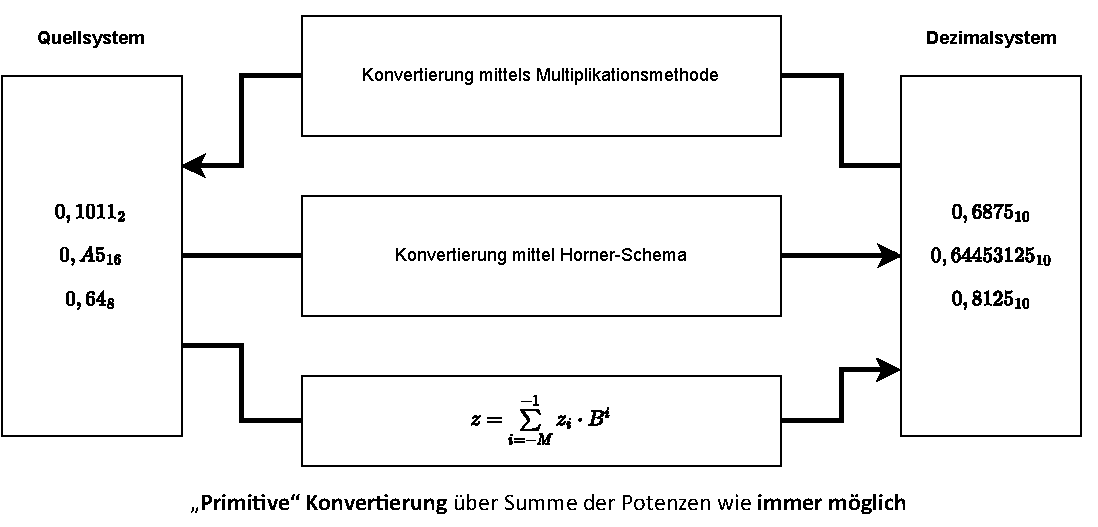
\includegraphics[height=.8\textheight]{fig/zahlensysteme_konvertierung_rational_echt.pdf}
\end{frame}

\begin{frame}{Konvertierung in das und aus dem Dezimalsystem}{Unechte Brüche}
  \centering
  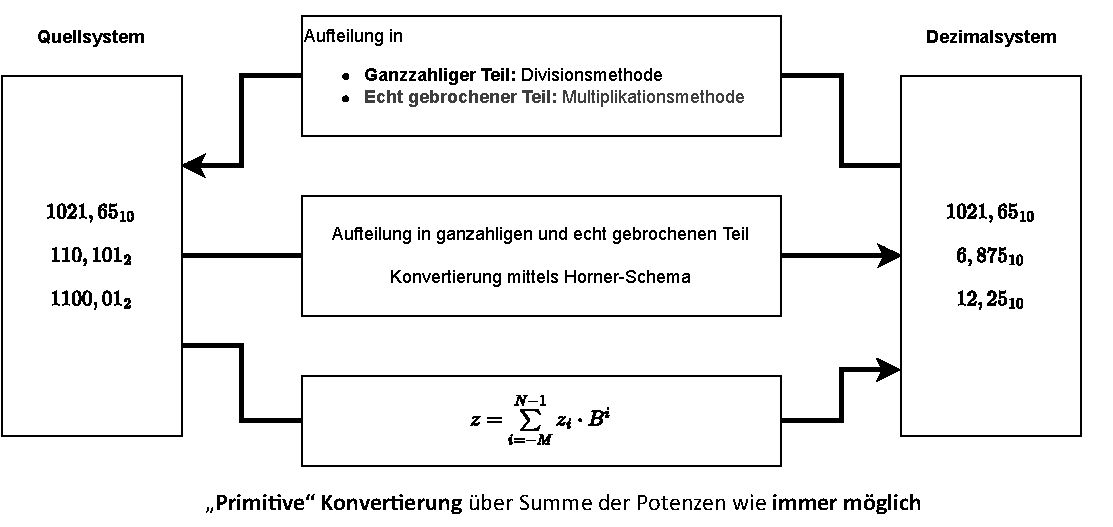
\includegraphics[height=.8\textheight]{fig/zahlensysteme_konvertierung_rational_unecht.pdf}
\end{frame}

\begin{frame}{Konvertierung in das und aus dem Dezimalsystem}{Beispiel I: Dezimalsystem \textrightarrow Dezimalsystem}
  \begin{align*}
    1021,65_{10} & = z_{-2} \cdot 10^{-2} + z_{-1} \cdot 10^{-1} + z_0 \cdot 10^0 + z_1 \cdot 10^1 + z_2 \cdot 10^2 + z_3 \cdot 10^3 \\
                 & = 5 \cdot 10^{-2} + 6 \cdot 10^{-1} + 1 \cdot 10^0 + 2 \cdot 10^1 + 0 \cdot 10^2 + 1 \cdot 10^3                   \\
                 & = 5 \cdot \frac{1}{100} + 6 \cdot \frac{1}{10} + 1 \cdot 1 + 2 \cdot 10 + 0 \cdot 100 + 1 \cdot 1000              \\
                 & = 5 \cdot 0,01 + 6 \cdot 0,1 + 1 \cdot 1 + 2 \cdot 10 + 0 \cdot 100 + 1 \cdot 1000                                \\
                 & = 0,05 + 0,6 + 1 + 20 + 0 + 1000                                                                                  \\
                 & = 1021,65_{10}
  \end{align*}
\end{frame}

\begin{frame}{Konvertierung in das und aus dem Dezimalsystem}{Beispiel II: Dualsystem \textrightarrow Dezimalsystem}
  \begin{align*}
    110,101_{2} & = z_{-3} \cdot 2^{-3} + z_{-2} \cdot 2^{-2} + z_{-1} \cdot 2^{-1} + z_0 \cdot 2^0 + z_1 \cdot 2^1 + z_2 \cdot 2^2 \\
                & = 1 \cdot 2^{-3} + 0 \cdot 2^{-2} + 1 \cdot 2^{-1} + 0 \cdot 2^0 + 1 \cdot 2^1 + 1 \cdot 2^2                      \\
                & = 1 \cdot \frac{1}{8} + 0 \cdot \frac{1}{4} + 1 \cdot \frac{1}{2} + 0 \cdot 1 + 1 \cdot 2 + 1 \cdot 4             \\
                & = 1 \cdot 0,125 + 0 \cdot 0,25 + 1 \cdot 0,5 + 0 \cdot 1 + 1 \cdot 2 + 1 \cdot 4                                  \\
                & = 0,125 + 0 + 0,5 + 0 + 2 + 4                                                                                     \\
                & = 6,625_{10}                                                                                                      \\
  \end{align*}
\end{frame}

\begin{frame}{Konvertierung in das und aus dem Dezimalsystem}{Beispiel III: Oktalsystem \textrightarrow Dezimalsystem}
  \begin{align*}
    0,64_{8} & = z_{-2} \cdot 8^{-2} + z_{-1} \cdot 8^{-1} + z_0 \cdot 8^0 \\
             & = 4 \cdot 8^{-2} + 6 \cdot 8^{-1} + 0 \cdot 8^0             \\
             & = 4 \cdot \frac{1}{64} + 6 \cdot \frac{1}{8} + 0 \cdot 1    \\
             & = 4 \cdot 0,015625 + 6 \cdot 0,125 + 0                      \\
             & = 0,0625 + 0,75 + 0                                         \\
             & = 0,8125_{10}
  \end{align*}
\end{frame}

\begin{frame}[t]{Konvertierung in das und aus dem Dezimalsystem}{Horner-Schema}
  Eine echt gebrochene Zahl $z$ im Basis-$B$-System lässt sich wie folgt mittels des Horner-Schemas darstellen:
  \[ z = \left( \left. \left. \ldots \left( z_{-M} \cdot \frac{1}{B} + z_{-M+1} \right) \cdot \frac{1}{B} + z_{-M+2} \right) \cdot \frac{1}{B} + \ldots + z_{-2} \right) \cdot \frac{1}{B} + z_{-1} \right) \cdot \frac{1}{B} \]
  Mit
  \begin{itemize}
    \item Basis $B$,
    \item $M$ Nachkommastellen,
    \item $z_i$ Ziffern $\left(0 \leq z_i < B\right)$,
  \end{itemize}
  \only<2>{
    \begin{exampleblock}{Beispiel 1: Oktalsystem \textrightarrow Dezimalsystem}
      \[ 0,64_{8} = \left( 4 \cdot \frac{1}{8} + 6 \right) \cdot \frac{1}{8} = \left( \frac{4}{8} + 6 \right) \cdot \frac{1}{8} = \left( \frac{4}{8} + \frac{48}{8} \right) \cdot \frac{1}{8} = \frac{52}{8} \cdot \frac{1}{8} = \frac{52}{64} = 0,8125_{10} \]
    \end{exampleblock}
  }
  \only<3>{
    \begin{exampleblock}{Beispiel 2: Dualsystem \textrightarrow Dezimalsystem}
      \[ 0,1011_{2} = \left( \left( \left( 1 \cdot \frac{1}{2} + 1 \right) \cdot \frac{1}{2} \right) \cdot \frac{1}{2} + 1 \right) \cdot \frac{1}{2} = \frac{11}{16} = 0,6875_{10} \]
    \end{exampleblock}
  }

\end{frame}

\begin{frame}[t]{Konvertierung echt gebrochener Zahlen aus dem Dezimalsystem}{Multiplikationsmethode}
  \begin{columns}
    \begin{column}{0.5\textwidth}
      \begin{block}{Verfahren}
        \begin{enumerate}
          \item Bilde $a \cdot B = y \mbox{ Überlauf } z$
                \begin{itemize}
                  \item[$y$] echt gebrochener Anteil
                  \item[$z$] ganzzahliger Anteil
                \end{itemize}
          \item Prüfe $y \neq 0$
                \begin{itemize}
                  \item Wenn $y \neq 0$
                        \begin{itemize}
                          \item Mache $y$ zum neuen $a$ und setze mit Schritt 1 fort
                        \end{itemize}
                  \item Wenn $y = 0$
                        \begin{itemize}
                          \item Beende die Berechnung
                          \item Die ermittelten Überlaufe $z$ sind die Ziffern des Ergebnisses in der Reihenfolge in der sie ermittelt wurden.
                        \end{itemize}
                \end{itemize}
        \end{enumerate}
      \end{block}
    \end{column}
    \begin{column}{0.5\textwidth}

      \only<2>{
        \begin{exampleblock}{Beispiel 1}
          \centering

          \begin{tabular}{rcccrrr}
            \toprule
            $a$                                   & $\cdot$ & $B$ & $=$ & $Ergebnis$ & $z$                             & $y$                                 \\
            \midrule
            0,125                                 & $\cdot$ & 2   & $=$ & 0.25       & \tikzmarknode{mult_line_1_z}{0} & \tikzmarknode{mult_line1_end}{0,25} \\
            \\
            \tikzmarknode{mult_line2_begin}{0,25} & $\cdot$ & 2   & $=$ & 0,5        & \tikzmarknode{mult_line_2_z}{0} & \tikzmarknode{mult_line2_end}{0,5}  \\
            \\
            \tikzmarknode{mult_line3_begin}{0,5}  & $\cdot$ & 2   & $=$ & 1.0        & \tikzmarknode{mult_line_3_z}{1} & 0,0                                 \\
            \bottomrule
          \end{tabular}
          \begin{tikzpicture}[remember picture, overlay]
            \draw[<-, thick] (mult_line2_begin.west) -| ++ (-.3,.8\baselineskip) -| ([xshift=-5]mult_line1_end.south east);
            \draw[<-, thick] (mult_line3_begin.west) -| ++ (-.48,.8\baselineskip) -| ([xshift=-5]mult_line2_end.south east);
            \draw[->, line width=2pt, color=red] ([xshift=3]mult_line_1_z.north east) -- ([xshift=3]mult_line_3_z.south east);
          \end{tikzpicture}
          \[ 0,125_{10} = 0,001_{2} \]
        \end{exampleblock}
      }
    \end{column}
  \end{columns}
\end{frame}

\begin{frame}[t]{Konvertierung echt gebrochener Zahlen aus dem Dezimalsystem}{Multiplikationsmethode -- Beispiele}
  \begin{columns}
    \begin{column}{0.5\textwidth}
      \begin{exampleblock}{Beispiel 2}
        \centering
        \begin{tabular}{rcccrrr}
          \toprule
          $a$    & $\cdot$ & $B$ & $=$ & $Ergebnis$ & $z$ & $y$   \\
          \midrule
          0,6875 & $\cdot$ & 2   & $=$ & 1,375      & 1   & 0,375 \\
          0,375  & $\cdot$ & 2   & $=$ & 0,75       & 0   & 0,75  \\
          0,75   & $\cdot$ & 2   & $=$ & 1,5        & 1   & 0,5   \\
          0,5    & $\cdot$ & 2   & $=$ & 1,0        & 1   & 0,0   \\
          \bottomrule
        \end{tabular}
        \[ 0,6875_{10} = 0,1011_{2} \]
      \end{exampleblock}
    \end{column}
    \begin{column}{0.5\textwidth}
      \begin{exampleblock}{Beispiel 3}
        \centering
        \begin{tabular}{rcccrrr}
          \toprule
          $a$  & $\cdot$ & $B$ & $=$ & $Ergebnis$ & $z$ & $y$ \\
          \midrule
          0,25 & $\cdot$ & 2   & $=$ & 0,5        & 0   & 0,5 \\
          0,5  & $\cdot$ & 2   & $=$ & 1,0        & 1   & 0,0 \\
          \bottomrule                                         \\
          \\
        \end{tabular}
        \[ 0,25_{10} = 0,01_{2} \]
      \end{exampleblock}
    \end{column}
  \end{columns}
\end{frame}

\begin{frame}{Konvertierung echt gebrochener Zahlen aus dem Dezimalsystem}{Multiplikationsmethode -- Periodische Zahlen}
  \begin{exampleblock}{Beispiel einer periodischen Zahl}
    \begin{columns}
      \begin{column}{0.7\textwidth}
        \centering
        \begin{tabular}{rcccrrr}
          \toprule
          $a$ & $\cdot$ & $B$ & $=$ & $Ergebnis$ & $z$        & $y$                           \\
          \midrule
          0,1 & $\cdot$ & 2   & $=$ & 0,2        & 0          & 0,2                           \\
          0,2 & $\cdot$ & 2   & $=$ & 0,4        & \textbf{0} & \textbf{\textcolor{red}{0,4}} \\
          0,4 & $\cdot$ & 2   & $=$ & 0,8        & \textbf{0} & 0,8                           \\
          0,8 & $\cdot$ & 2   & $=$ & 1,6        & \textbf{1} & 0,6                           \\
          0,6 & $\cdot$ & 2   & $=$ & 1,2        & \textbf{1} & 0,2                           \\
          0,2 & $\cdot$ & 2   & $=$ & 0,4        & 0          & \textbf{\textcolor{red}{0,4}} \\
          \bottomrule
        \end{tabular}
      \end{column}
      \begin{column}{0.3\textwidth}
        \[ 0,1_{10} = 0,0\overline{0011}_{2} \]
      \end{column}
    \end{columns}
  \end{exampleblock}
  \begin{alertblock}{Unterschiedliche Periodeneigenschaft}
    Manche Zahlen, die in einem System eine endliche Darstellung haben, haben in einem anderen System eine periodische Darstellung.

  \end{alertblock}
\end{frame}

\begin{frame}{Konvertierung unecht gebrochener Zahlen aus dem Dezimalsystem}{Kombination aus Divisionsmethode und Multiplikationsmethode}

  \vspace{-.3\baselineskip}
  \begin{block}{Verfahren}
    Bei der Konvertierung unecht gebrochener Zahlen wird die Zahl in den ganzzahligen und den echt gebrochenen Anteil zerlegt.
    \begin{itemize}
      \item Der ganzzahlige Anteil wird mit der Divisionsmethode konvertiert.
      \item Der echt gebrochene Anteil wird mit der Multiplikationsmethode konvertiert.
    \end{itemize}

  \end{block}
  \vspace{-.1\baselineskip}
  \begin{exampleblock}{Beispiel}
    \begin{columns}
      \begin{column}{0.12\textwidth}
        \[ 12,25_{10} \]
        \[ =  \]
        \[ 1100,01_{2} \]
      \end{column}
      \begin{column}{0.4\textwidth}
        \centering
        Ganzzahliger Anteil
        \begin{tabular}{rcrcrcr}
          \toprule
          $a$ & $\div$ & $B$ & $=$ & $x$ & Rest & y                                          \\
          \midrule
          12  & $\div$ & 2   & $=$ & 6   & Rest & \tikzmarknode{combined_division_top}{0}    \\
          6   & $\div$ & 2   & $=$ & 3   & Rest & 0                                          \\
          3   & $\div$ & 2   & $=$ & 1   & Rest & 1                                          \\
          1   & $\div$ & 2   & $=$ & 0   & Rest & \tikzmarknode{combined_division_bottom}{1} \\
          \bottomrule
        \end{tabular}

      \end{column}
      \begin{column}{0.42\textwidth}
        \centering
        Echt gebrochener Anteil
        \begin{tabular}{rcccrrr}
          \toprule
          $a$  & $\cdot$ & $B$ & $=$ &     & $z$                                    & $y$ \\
          \midrule
          0,25 & $\cdot$ & 2   & $=$ & 0,5 & \tikzmarknode{combined_mult_top}{0}    & 0,5 \\
          0,5  & $\cdot$ & 2   & $=$ & 1,0 & \tikzmarknode{combined_mult_bottom}{1} & 0,0 \\
          \bottomrule
        \end{tabular}
      \end{column}
      \begin{tikzpicture}[remember picture, overlay]
        \draw[<-, thick] ([xshift=3pt]combined_division_top.north east) --([xshift=3pt]combined_division_bottom.south east);
        \draw[->, thick] ([xshift=3pt]combined_mult_top.north east) --([xshift=3pt]combined_mult_bottom.south east);
      \end{tikzpicture}
    \end{columns}
  \end{exampleblock}

\end{frame}

\begin{frame}{Darstellung reeller Zahlen}
  \begin{alertblock}{Problem}
    \centering
    Wo ist das Komma?
    \[ 010101011110011011110101 \]
  \end{alertblock}
  \begin{block}{Systeme}
    \begin{itemize}
      \item Darstellung als Bruch zweier Ganzzahlen (nur für rationale Zahlen)
      \item Darstellung mit fixem Komma (Festkomma)
      \item Darstellung mit variablen Komma (Gleitkomma)
    \end{itemize}
  \end{block}

\end{frame}

\begin{frame}[t]{Fixkomma/Festkomma (fixed-point Numbers)}{Methode}

  \begin{block}{Idee}
    \begin{itemize}
      \item Komma an fester Stelle und wie mit ganzen Zahlen rechnen
      \item Bei Multiplikation und Division muss das Ergebnis skaliert werden (Komma verschieben)
    \end{itemize}
  \end{block}

  \only<2>{
    \begin{exampleblock}{Beispiele Addition}
      \begin{columns}[T] % Added T option for top alignment and center alignment
        \begin{column}{0.25\textwidth}
          \[
            \begin{array}{lccc}
                & 1 & 2      & 5 \\
              + & 2 & 0      & 5 \\
                &   & {}_{1} &   \\
              \hline
                & 3 & 3      & 0
            \end{array}
          \]
        \end{column}
        \begin{column}{0.25\textwidth}
          \[
            \begin{array}{lcccc}
                & 1 & , & 2      & 5 \\
              + & 2 & , & 0      & 5 \\
                &   &   & {}_{1} &   \\
              \hline
                & 3 & , & 3      & 0
            \end{array}
          \]
        \end{column}
        \begin{column}{0.5\textwidth}
          \vspace{\baselineskip}
          \[
            \begin{array}{lcccccccc}
                & 0 & 1 & , & 0 & 1 & 0 & 0 & 0 \\
              + & 1 & 0 & , & 1 & 0 & 1 & 0 & 0 \\
                &   &   &   &   &   &   &   &   \\
              \hline
                & 1 & 1 & , & 1 & 1 & 1 & 0 & 0
            \end{array}
          \]
        \end{column}
      \end{columns}
    \end{exampleblock}
  }
  \only<3>{
    \begin{exampleblock}{Beispiel Multiplikation}
      \begin{columns}
        \begin{column}{0.5\textwidth}
          \[
            \begin{array}{lcccc}
              1 & 6 & $\cdot$ & 2 & 4 \\
                &   & 3       & 2 &   \\
                &   &         & 6 & 4 \\
              \hline
                &   & 3       & 8 & 4
            \end{array}
          \]
        \end{column}
        \begin{column}{0.5\textwidth}
          \[
            \begin{array}{lccccccc}
              1 & , & 6 & $\cdot$ & 2 & , & 4     \\
                &   &   &         & 3 & , & 2 &   \\
                &   &   &         & 0 & , & 6 & 4 \\
              \hline
                &   &   &         & 3 & , & 8 & 4
            \end{array}
          \]
        \end{column}
      \end{columns}
    \end{exampleblock}
  }

\end{frame}


\begin{frame}[t]{Fixkomma/Festkomma (fixed-point Numbers)}{Technische Umsetzung}
  16-Bit-Zahl mit 8 Bit vor und 8 Bit nach dem Komma:
  \small
  \[
    \begin{array}{lccccccccccccccccc}
      Zahl   & 0   & 1   & 0   & 0   & 0   & 1   & 1   & 0   & , & 1           & 0           & 1           & 1            & 0            & 1            & 1             & 1             \\
      \hline
      Bit    & 0   & 1   & 2   & 3   & 4   & 5   & 6   & 7   & , & 8           & 9           & 10          & 11           & 12           & 13           & 14            & 15            \\
      \hline
      Ziffer & z_7 & z_6 & z_5 & z_4 & z_3 & z_2 & z_1 & z_0 & , & z_{-1}      & z_{-2}      & z_{-3}      & z_{-4}       & z_{-5}       & z_{-6}       & z_{-7}        & z_{-8}        \\
      Wert   & 128 & 64  & 32  & 16  & 8   & 4   & 2   & 1   & , & \frac{1}{2} & \frac{1}{4} & \frac{1}{8} & \frac{1}{16} & \frac{1}{32} & \frac{1}{64} & \frac{1}{128} & \frac{1}{256}
    \end{array}
  \]
  \only<1>{
    \begin{block}{Konventionen}
      \begin{itemize}
        \item Zahl $z$ hat $N$ Stellen ($0$ bis $N-1$) vor und $M$ Stellen ($-1$ bis $-M$) nach dem Komma
        \item der Dezimalpunkt (das Komma) steht implizit immer an einer bestimmten festgelgten Stelle und wird nicht mitgespeichert
      \end{itemize}
    \end{block}
  }
  \only<2>{
    \begin{block}{UMrechnung Bitmuster in Zahl}
      \begin{enumerate}
        \item Bitmuster als ganze Zahl interpretieren

              \[0100011010110111_{2} = 18 103_{10}\]
        \item Division durch den Wert $2^{M}$, wobei $M$ die Anzahl der Bits nach dem Komma ist
              \[
                \frac{18 103}{2^{8}} = \frac{18 103}{256} = 70,71484735
              \]
      \end{enumerate}


    \end{block}
  }
\end{frame}


\begin{frame}[t]{Fixkomma/Festkomma (fixed-point Numbers)}{Vor- und Nachteile}
  \begin{block}{Vorteile}
    \begin{itemize}
      \item Einfache und schnelle Rechenoperationen
      \item Geringer Speicherbedarf
    \end{itemize}
  \end{block}

  \begin{block}{Nachteile}
    \begin{itemize}
      \item Eingeschränkter Wertebereich
      \item Fehlende Flexibilität (z.~B. gleichzeitige Speicherung sowohl sehr großer als auch sehr kleiner Zahlen)
      \item Überlaufgefahr bei Multiplikation und Division
    \end{itemize}
  \end{block}
\end{frame}

\begin{frame}{Fließkommazahlen}
  \begin{columns}[T]
    \begin{column}{0.5\textwidth}
      \begin{block}{Idee}
        \begin{itemize}
          \item Bewegliches/gleitendes Komma
          \item Jede reelle Zahl kann als Gleitkommazahl dargestellt werden
                \[ z = a \cdot B ^ e \mbox{ mit } 1 \leq a \leq B \]
                \begin{itemize}
                  \item \(a\) ist die Mantisse
                  \item \(B\) ist die Basis
                  \item \(e\) ist der Exponent
                \end{itemize}
          \item funktioniert für jede Basis \(B\geq 2\)
        \end{itemize}
      \end{block}
    \end{column}
    \begin{column}{0.5\textwidth}
      \begin{block}{Wissenschaftliche Schreibweise}
        \begin{itemize}
          \item Normalisierte Exponentialschreibweise
          \item Multiplikation: Multipliktion der Basen und Addition der Exponenten
          \item Division: Division der Basen und Subtraktion der Exponenten
        \end{itemize}
      \end{block}
      \begin{exampleblock}{Normalisierung}
        \begin{itemize}
          \item \(0.123\) ist nicht normalisiert
          \item \(1.23 \cdot 10^{-1}\) ist normalisiert
          \item \(123 \) ist nicht normalisiert
          \item \(1.23 \cdot 10^2\) ist normalisiert
        \end{itemize}

      \end{exampleblock}
    \end{column}
  \end{columns}

\end{frame}

\begin{frame}{Fließkommazahlen}{IEEE Standard 754}
  \begin{block}{Standard zur Gleitkommadarstellung (1985)}
    \textbf{I}nstitute of \textbf{E}lectrical and \textbf{E}lectronics \textbf{E}ngineers Standard 754
  \end{block}
  \begin{alertblock}{Vorsicht}
    \centering
    Oder: Warum \( 0,1 + 0,1 + 0,1 \neq 0,3 \)?
  \end{alertblock}
\end{frame}

\begin{frame}{Fließkommazahlen}{IEEE Standard 754 -- Darstellung}
  \setlength{\tabcolsep}{0.2em}
  \[ z = a \cdot 2^{x} \]
  \begin{tabular}{c|cccccccc|ccccccccccccccccccccccc}
    \toprule
    0                               & 1                                      & 2                                      & 3 & 4 & 5 & 6 & 7 & 8 & 9 & 10 & 11 & 12 & 13 & 14 & 15 & 16 & 17 & 18 & 19 & 20 & 21 & 22 & 23 & 24 & 25 & 26 & 27 & 28 & 29 & 30 & 31 \\
    \multicolumn{1}{c|}{\textbf{S}} & \multicolumn{8}{c|}{\textbf{Exponent}} & \multicolumn{23}{c}{\textbf{Mantisse}}                                                                                                                                           \\
    \midrule
  \end{tabular}

  \begin{itemize}
    \item Vorzeichenbit
          \begin{itemize}
            \item 0 = positiv
            \item 1 = negativ
          \end{itemize}
    \item Mantisse

          Zahl wird normalisiert abgespeichert. D.h. es steht eine 1 vor dem Komma. Diese 1 wird nicht gespeichert.
    \item Exponent
          \begin{itemize}
            \item \(2 ^ {8} = 256 darstellbare Werte\)
            \item Exponenten \( 0000 0000 \) und \( 1111 1111 \) sind reserviert
            \item Exponent hat den Wertebereich \([-126, 127]\), wird als \(x - 127\) gespeichert (Bias)
          \end{itemize}
  \end{itemize}


\end{frame}

\begin{frame}{Fließkommazahlen}{IEEE Standard 754 -- Vergleichbarkeit}

  \begin{block}{Warum der Bias?}
    Der Bias macht den Größenvergleich von Gleitkommazahlen einfacher.

    \begin{itemize}
      \item Bitweiser Vergleich zweier Gleitkommazahlen $a$ und $b$ von links nach rechts.
      \item Die Zahl die am weitesten links eine 1 hat (ausgenommen Vorzeichenbit) ist die größere Zahl.
    \end{itemize}
  \end{block}

  \setlength{\tabcolsep}{0.2em}
  \begin{tabular}{c|cccccccc|ccccccccccccccccccccccc}
    \toprule
    0 & 1                            & 2 & 3 & 4 & 5 & 6 & 7 & 8 & 9                           & 10 & 11 & 12 & 13 & 14 & 15 & 16 & 17 & 18 & 19 & 20 & 21 & 22 & 23 & 24 & 25 & 26 & 27 & 28 & 29 & 30 & 31 \\
    \midrule
    0 & \tikzmarknode{ffcomp_top}{1} & 0 & 0 & 0 & 0 & 0 & 1 & 0 & \multicolumn{23}{c}{23 Bit}                                                                                                               \\
    0 & \tikzmarknode{ffcomp_bot}{0} & 1 & 0 & 0 & 0 & 0 & 1 & 0 & \multicolumn{23}{c}{23 Bit}                                                                                                               \\
    \bottomrule
  \end{tabular}

  \begin{tikzpicture}[remember picture, overlay]
    \draw[red, thick] ([shift={(-0.02,0.15)}]ffcomp_top.north west) rectangle ([shift={(0.02,-0.15)}]ffcomp_bot.south east);
  \end{tikzpicture}

\end{frame}

\begin{frame}{Fließkommazahlen}{IEEE Standard 754 -- Beispiel}
  \[ +100_{10} = 0110 0100_{2} = + 1.\tikzmarknode{b1mant}{1001} \cdot 2^{\tikzmarknode{b1exp}{6}} \]

  Exponent:
  \[ x = 127_{10} + 6_{10} = 133_{10} = 1000 0101_{2} \]

  \begin{tikzpicture}[remember picture, overlay]
    \draw[blue, thick] ([shift={(-0.05,0.1)}]b1mant.north west) rectangle ([shift={(0.05,-0.1)}]b1mant.south east);
    \draw[red, thick] ([shift={(-0.05,0.1)}]b1exp.north west) rectangle ([shift={(0.05,-0.1)}]b1exp.south east);
  \end{tikzpicture}

  \setlength{\tabcolsep}{0.2em}
  \begin{tabular}{c|cccccccc|ccccccccccccccccccccccc}
    \toprule
    0                               & 1                                      & 2                                      & 3 & 4 & 5 & 6 & 7 & 8 & 9 & 10 & 11 & 12 & 13 & 14 & 15 & 16 & 17 & 18 & 19 & 20 & 21 & 22 & 23 & 24 & 25 & 26 & 27 & 28 & 29 & 30 & 31 \\
    \multicolumn{1}{c|}{\textbf{S}} & \multicolumn{8}{c|}{\textbf{Exponent}} & \multicolumn{23}{c}{\textbf{Mantisse}}                                                                                                                                           \\
    \midrule
    0                               & 1                                      & 0                                      & 0 & 0 & 0 & 1 & 0 & 1 & 1 & 0  & 0  & 1  & 0  & 0  & 0  & 0  & 0  & 0  & 0  & 0  & 0  & 0  & 0  & 0  & 0  & 0  & 0  & 0  & 0  & 0  & 0  \\
    \bottomrule
  \end{tabular}
\end{frame}

\begin{frame}{Fließkommazahlen}{IEEE Standard 754 -- Obergrenze}
  Größte darstellbare positive Zahl:
  \[1.11 \ldots 1 \cdot 2^{254-127} = 1.11 \ldots 1 \cdot 2^{127} = (2 - 2^{-23}) \cdot 2^{127} = 2^{127} - 2^{104}
    \approx 1.701 \cdot 10^{38}\]

  \setlength{\tabcolsep}{0.2em}
  \begin{tabular}{c|cccccccc|ccccccccccccccccccccccc}
    \toprule
    0                               & 1                                      & 2                                      & 3 & 4 & 5 & 6 & 7 & 8 & 9 & 10 & 11 & 12 & 13 & 14 & 15 & 16 & 17 & 18 & 19 & 20 & 21 & 22 & 23 & 24 & 25 & 26 & 27 & 28 & 29 & 30 & 31 \\
    \multicolumn{1}{c|}{\textbf{S}} & \multicolumn{8}{c|}{\textbf{Exponent}} & \multicolumn{23}{c}{\textbf{Mantisse}}                                                                                                                                           \\
    \midrule
    0                               & 1                                      & 1                                      & 1 & 1 & 1 & 1 & 1 & 0 & 1 & 1  & 1  & 1  & 1  & 1  & 1  & 1  & 1  & 1  & 1  & 1  & 1  & 1  & 1  & 1  & 1  & 1  & 1  & 1  & 1  & 1  & 1  \\
    \bottomrule
  \end{tabular}

\end{frame}

\begin{frame}{Fließkommazahlen}{IEEE Standard 754 -- Untergrenze}
  Kleinste darstellbare positive Zahl:
  \[1.00 \ldots0 \cdot 2^{1-127} = 1.00 \ldots0 \cdot 2^{-126} = 2^{-126} = 1.401 \cdot 10^{-45}\]

  \setlength{\tabcolsep}{0.2em}
  \begin{tabular}{c|cccccccc|ccccccccccccccccccccccc}
    \toprule
    0                               & 1                                      & 2                                      & 3 & 4 & 5 & 6 & 7 & 8 & 9 & 10 & 11 & 12 & 13 & 14 & 15 & 16 & 17 & 18 & 19 & 20 & 21 & 22 & 23 & 24 & 25 & 26 & 27 & 28 & 29 & 30 & 31 \\
    \multicolumn{1}{c|}{\textbf{S}} & \multicolumn{8}{c|}{\textbf{Exponent}} & \multicolumn{23}{c}{\textbf{Mantisse}}                                                                                                                                           \\
    \midrule
    0                               & 0                                      & 0                                      & 0 & 0 & 0 & 0 & 0 & 1 & 0 & 0  & 0  & 0  & 0  & 0  & 0  & 0  & 0  & 0  & 0  & 0  & 0  & 0  & 0  & 0  & 0  & 0  & 0  & 0  & 0  & 0  & 0  \\
    \bottomrule
  \end{tabular}
\end{frame}


\begin{frame}{Fließkommazahlen}{IEEE Standard 754 -- Reservierte Werte}
  \centering
  \begin{tabular}{lccl}
    \toprule{Spezielle Werte} & \textbf{Exponent} & \textbf{Mantisse} & \textbf{Bedeutung} \\
    \midrule
    \textbf{Null}             & 0000 0000         & 0                 & \(+0\)             \\
    \textbf{Unendlichkeit}    & 1111 1111         & 0                 & \(+\infty\)        \\
    \textbf{NaN}              & 1111 1111         & $\neq 0$          & Not a Number       \\
    \textbf{Denormalized}     & 0000 0000         & $\neq 0$          & führende 0 statt 1 \\
    \bottomrule
  \end{tabular}
\end{frame}

% End document
\end{document}
